        %%******************************************%%
        %%                                          %%
        %%        Modello di tesi di laurea         %%
        %%            di Andrea Giraldin            %%
        %%                                          %%
        %%             2 novembre 2012              %%
        %%                                          %%
        %%******************************************%%


% I seguenti commenti speciali impostano:
% 1. 
% 2. PDFLaTeX come motore di composizione;
% 3. tesi.tex come documento principale;
% 4. il controllo ortografico italiano per l'editor.

% !TEX encoding = UTF-8
% !TEX TS-program = pdflatex
% !TEX root = tesi.tex
% !TEX spellcheck = it-IT

% PDF/A filecontents
\RequirePackage{filecontents}
\begin{filecontents*}{\jobname.xmpdata}
  \Title{Document’s title}
  \Author{Author’s name}
  \Language{it-IT}
  \Subject{The abstract, or short description.}
  \Keywords{keyword1\sep keyword2\sep keyword3}
\end{filecontents*}

\documentclass[10pt,                    % corpo del font principale
               a4paper,                 % carta A4
               twoside,                 % impagina per fronte-retro
               openright,               % inizio capitoli a destra
               english,                 
               italian,                 
               ]{book}    

%**************************************************************
% Importazione package
%************************************************************** 

\PassOptionsToPackage{dvipsnames}{xcolor} % colori PDF/A

\usepackage{colorprofiles}

\usepackage[a-2b,mathxmp]{pdfx}[2018/12/22]
                                        % configurazione PDF/A
                                        % validare in https://www.pdf-online.com/osa/validate.aspx

%\usepackage{amsmath,amssymb,amsthm}    % matematica

\usepackage[T1]{fontenc}                % codifica dei font:
                                        % NOTA BENE! richiede una distribuzione *completa* di LaTeX

\usepackage[utf8]{inputenc}             % codifica di input; anche [latin1] va bene
                                        % NOTA BENE! va accordata con le preferenze dell'editor

\usepackage[english, italian]{babel}    % per scrivere in italiano e in inglese;
                                        % l'ultima lingua (l'italiano) risulta predefinita

\usepackage{bookmark}                   % segnalibri

\usepackage{caption}                    % didascalie

\usepackage{chngpage,calc}              % centra il frontespizio

\usepackage{csquotes}                   % gestisce automaticamente i caratteri (")

\usepackage{emptypage}                  % pagine vuote senza testatina e piede di pagina

\usepackage{epigraph}			% per epigrafi

\usepackage{eurosym}                    % simbolo dell'euro

%\usepackage{indentfirst}               % rientra il primo paragrafo di ogni sezione

\usepackage{graphicx}                   % immagini

\usepackage{hyperref}                   % collegamenti ipertestuali

\usepackage[binding=5mm]{layaureo}      % margini ottimizzati per l'A4; rilegatura di 5 mm
\usepackage{float}
\usepackage{listings}                   % codici

\usepackage{microtype}                  % microtipografia
\usepackage{multirow}
\usepackage{mparhack,fixltx2e,relsize}  % finezze tipografiche

\usepackage{nameref}                    % visualizza nome dei riferimenti                                      
\usepackage[font=small]{quoting}        % citazioni

\usepackage{subfig}                     % sottofigure, sottotabelle

\usepackage[italian]{varioref}          % riferimenti completi della pagina

\usepackage{booktabs}                   % tabelle                                       
\usepackage{tabularx}                   % tabelle di larghezza prefissata                                    
\usepackage{longtable}                  % tabelle su più pagine                                        
\usepackage{ltxtable}                   % tabelle su più pagine e adattabili in larghezza

\usepackage[toc, acronym]{glossaries}   % glossario
                                        % per includerlo nel documento bisogna:
                                        % 1. compilare una prima volta tesi.tex;
                                        % 2. eseguire: makeindex -s tesi.ist -t tesi.glg -o tesi.gls tesi.glo
                                        % 3. eseguire: makeindex -s tesi.ist -t tesi.alg -o tesi.acr tesi.acn
                                        % 4. compilare due volte tesi.tex.

\usepackage[backend=biber,style=verbose-ibid,hyperref,backref]{biblatex}
                                        % eccellente pacchetto per la bibliografia; 
                                        % produce uno stile di citazione autore-anno; 
                                        % lo stile "numeric-comp" produce riferimenti numerici
                                        % per includerlo nel documento bisogna:
                                        % 1. compilare una prima volta tesi.tex;
                                        % 2. eseguire: biber tesi
                                        % 3. compilare ancora tesi.tex.

%**************************************************************
% file contenente le impostazioni della tesi
%**************************************************************

%**************************************************************
% Frontespizio
%**************************************************************

% Autore
\newcommand{\myName}{Luciano Wu}
\newcommand{\myTitle}{Sviluppo di una web-app per la gestione degli ordini di ristoranti}

% Tipo di tesi                   
\newcommand{\myDegree}{Tesi di laurea}

% Università             
\newcommand{\myUni}{Università degli Studi di Padova}

% Facoltà       
\newcommand{\myFaculty}{Corso di Laurea in Informatica}

% Dipartimento
\newcommand{\myDepartment}{Dipartimento di Matematica "Tullio Levi-Civita"}

% Titolo del relatore
\newcommand{\profTitle}{Prof.}

% Relatore
\newcommand{\myProf}{Francesco Ranzato}

% Luogo
\newcommand{\myLocation}{Padova}

% Anno accademico
\newcommand{\myAA}{2021-2022}

% Data discussione
\newcommand{\myTime}{Dicembre 2022}


%**************************************************************
% Impostazioni di impaginazione
% see: http://wwwcdf.pd.infn.it/AppuntiLinux/a2547.htm
%**************************************************************

\setlength{\parindent}{14pt}   % larghezza rientro della prima riga
\setlength{\parskip}{0pt}   % distanza tra i paragrafi


%**************************************************************
% Impostazioni di biblatex
%**************************************************************
\bibliography{bibliografia} % database di biblatex 

\defbibheading{bibliography} {
    \cleardoublepage
    \phantomsection 
    \addcontentsline{toc}{chapter}{\bibname}
    \chapter*{\bibname\markboth{\bibname}{\bibname}}
}

\setlength\bibitemsep{1.5\itemsep} % spazio tra entry

\DeclareBibliographyCategory{opere}
\DeclareBibliographyCategory{web}

\addtocategory{opere}{womak:lean-thinking}
\addtocategory{web}{site:agile-manifesto}

\defbibheading{opere}{\section*{Riferimenti bibliografici}}
\defbibheading{web}{\section*{Siti Web consultati}}


%**************************************************************
% Impostazioni di caption
%**************************************************************
\captionsetup{
    tableposition=top,
    figureposition=bottom,
    font=small,
    format=hang,
    labelfont=bf
}

%**************************************************************
% Impostazioni di glossaries
%**************************************************************
\makeglossaries

%**************************************************************
% Acronimi
%**************************************************************


\newacronym[description={\glslink{apig}{Application Program Interface}}]
    {api}{API}{Application Program Interface}
\newacronym[description={\glslink{urlg}{Uniform Resource Locator}}]
    {url}{URL}{Uniform Resource Locator}
\newacronym[description={\glslink{voipg}{Voice over Internet Protocol}}]
    {VoiP}{Voice over Internet Protocol}
\newacronym[description={\glslink{restg}{Representational state transfer}}]
    {restg}{Representational state transfer}



%**************************************************************
% Glossario
%**************************************************************
%\renewcommand{\glossaryname}{Glossario}

\newglossaryentry{restg}
{
    name=\glslink{restg}{REST},
    text=REST,
    sort=REST,
    description={è uno stile architetturale per sistemi distribuiti. L'espressione "representational state transfer" e il suo acronimo, REST, fu introdotto nel 2000 nella tesi di dottorato di Roy Fielding e vennero rapidamente adottati dalla comunità di sviluppatori Internet. I metodi più utilizzati sono: GET, POST, PUT, PATCH e DELETE}
}
\newglossaryentry{gitg}{
    name=\glslink{gitg}{Git},
    text=Git,
    sort=git,
    description={un software per il controllo di versionamento per lo sviluppo delle applicazioni, nato nel 2005. Permette di creare rami e unire i rami, per un grande progetto che deve iniziare un implementazione di una nuova funzione si può creare un ramo feature e lavorare su questo ramo per mantenere il corretto funzionamento del programma nel ramo main, una volta che la feature è tutta finita lo si può fare il merge nel main del progetto}}

\newglossaryentry{apig}
{
    name=\glslink{apig}{API},
    text=API,
    sort=api,
    description={in informatica con il termine \emph{Application Programming Interface API} (ing. interfaccia di programmazione di un'applicazione) si indica ogni insieme di procedure disponibili al programmatore, di solito raggruppate a formare un set di strumenti specifici per l'espletamento di un determinato compito all'interno di un certo programma. La finalità è ottenere un'astrazione, di solito tra l'hardware e il programmatore o tra software a basso e quello ad alto livello semplificando così il lavoro di programmazione}
}

\newglossaryentry{urlg}
{
    name=\glslink{urlg}{url},
    text=URL,
    sort=URL,
    description={è una sequenza di caratteri che identifica univocamente l'indirizzo di una risorsa su una rete di computer, come ad esempio una pagina web, tipicamente presente su un host server e resa accessibile a un client. Un esempio di URL famoso può essere 'www.google.com'
    }
}
\newglossaryentry{responsiveg}
{
    name=\glslink{responsiveg}{responsive},
    text=responsive,
    sort=responsive,
    description={indica una tecnica di web design per la realizzazione di siti in grado di adattarsi graficamente in modo automatico al dispositivo coi quali vengono visualizzati, come computer, cellulare, monitor e TV, riducendo al minimo la necessità dell'utente di ridimensionare e scorrere i contenuti
    }
}
\newglossaryentry{mascherag}
{
    name=\glslink{mascherag}{maschera},
    text=maschera,
    sort=maschera,
    description={indica interfaccia che viene viene visualizzato all'utente}
}
\newglossaryentry{backendg}
{
    name=\glslink{backendg}{back-end},
    text=back-end,
    sort=back-end,
    description={parte del software che elabora i dati generati dal front-end e comunica con il data-base per scrive e leggere dati}
}
\newglossaryentry{frontendg}
{
    name=\glslink{frontendg}{front-end},
    text=front-end,
    sort=front-end,
    description={è la parte di un sistema software che gestisce l'interazione con l'utente o con sistemi esterni che producono dati di ingresso, comuni con il back-end tramite le chiamate REST}
}
% \newglossaryentry{asd}
% {
%     name=\glslink{asd},
%     text=asd,
%     sort=asd,
%     description={}
% }

\newglossaryentry{voipg}{
    name=\glslink{voipg}{VoiP},
    text=VoiP,
    sort=Voip,
    description={in telecomunicazioni e informatica, indica una tecnologia che rende possibile effettuare una conversazione, analoga a quella che si potrebbe ottenere con una rete telefonica, sfruttando una connessione Internet o una qualsiasi altra rete di telecomunicazioni dedicata a commutazione di pacchetto, che utilizzi il protocollo IP senza connessione per il trasporto dati}}



\newglossaryentry{Springg}{
    name=\glslink{Springg}{Spring},
    text=Spring,
    sort=spring,
    description={un framework open source per lo sviluppo delle applicazioni su piattaforma Java, nato nel 2002. Le sue pricipali punti di forza sono: flessibilità ,modularità, elevata testabilità e una grande community. Per fare questo spring si basa sui seguenti principi: dependency injection}}

 % database di termini


%**************************************************************
% Impostazioni di graphicx
%**************************************************************
\graphicspath{{immagini/}} % cartella dove sono riposte le immagini


%**************************************************************
% Impostazioni di hyperref
%**************************************************************
\hypersetup{
    %hyperfootnotes=false,
    %pdfpagelabels,
    %draft,	% = elimina tutti i link (utile per stampe in bianco e nero)
    colorlinks=true,
    linktocpage=true,
    pdfstartpage=1,
    pdfstartview=,
    % decommenta la riga seguente per avere link in nero (per esempio per la stampa in bianco e nero)
    %colorlinks=false, linktocpage=false, pdfborder={0 0 0}, pdfstartpage=1, pdfstartview=FitV,
    breaklinks=true,
    pdfpagemode=UseNone,
    pageanchor=true,
    pdfpagemode=UseOutlines,
    plainpages=false,
    bookmarksnumbered,
    bookmarksopen=true,
    bookmarksopenlevel=1,
    hypertexnames=true,
    pdfhighlight=/O,
    %nesting=true,
    %frenchlinks,
    urlcolor=webbrown,
    linkcolor=RoyalBlue,
    citecolor=webgreen,
    %pagecolor=RoyalBlue,
    %urlcolor=Black, linkcolor=Black, citecolor=Black, %pagecolor=Black,
    pdftitle={\myTitle},
    pdfauthor={\textcopyright\ \myName, \myUni, \myFaculty},
    pdfsubject={},
    pdfkeywords={},
    pdfcreator={pdfLaTeX},
    pdfproducer={LaTeX}
}

%**************************************************************
% Impostazioni di itemize
%**************************************************************
% \renewcommand{\labelitemi}{$\ast$}

%\renewcommand{\labelitemi}{$\bullet$}
%\renewcommand{\labelitemii}{$\cdot$}
%\renewcommand{\labelitemiii}{$\diamond$}
%\renewcommand{\labelitemiv}{$\ast$}


%**************************************************************
% Impostazioni di listings
%**************************************************************
\lstset{
    language=[LaTeX]Tex,%C++,
    keywordstyle=\color{RoyalBlue}, %\bfseries,
    basicstyle=\small\ttfamily,
    %identifierstyle=\color{NavyBlue},
    commentstyle=\color{Green}\ttfamily,
    stringstyle=\rmfamily,
    numbers=none, %left,%
    numberstyle=\scriptsize, %\tiny
    stepnumber=5,
    numbersep=8pt,
    showstringspaces=false,
    breaklines=true,
    frameround=ftff,
    frame=single
} 


%**************************************************************
% Impostazioni di xcolor
%**************************************************************
\definecolor{webgreen}{rgb}{0,.5,0}
\definecolor{webbrown}{rgb}{.6,0,0}


%**************************************************************
% Altro
%**************************************************************

\newcommand{\omissis}{[\dots\negthinspace]} % produce [...]

% eccezioni all'algoritmo di sillabazione
\hyphenation
{
    ma-cro-istru-zio-ne
    gi-ral-din
}

\newcommand{\sectionname}{sezione}
\addto\captionsitalian{\renewcommand{\figurename}{Figura}
                       \renewcommand{\tablename}{Tabella}}

\newcommand{\glsfirstoccur}{\ap{{[g]}}}

\newcommand{\intro}[1]{\emph{\textsf{#1}}}

%**************************************************************
% Environment per ``rischi''
%**************************************************************
\newcounter{riskcounter}                % define a counter
\setcounter{riskcounter}{0}             % set the counter to some initial value

%%%% Parameters
% #1: Title
\newenvironment{risk}[1]{
    \refstepcounter{riskcounter}        % increment counter
    \par \noindent                      % start new paragraph
    \textbf{\arabic{riskcounter}. #1}   % display the title before the 
                                        % content of the environment is displayed 
}{
    \par\medskip
}

\newcommand{\riskname}{Rischio}

\newcommand{\riskdescription}[1]{\textbf{\\Descrizione:} #1.}

\newcommand{\risksolution}[1]{\textbf{\\Soluzione:} #1.}

%**************************************************************
% Environment per ``use case''
%**************************************************************
\newcounter{usecasecounter}             % define a counter
\setcounter{usecasecounter}{0}          % set the counter to some initial value

%%%% Parameters
% #1: ID
% #2: Nome
\newenvironment{usecase}[2]{
    \renewcommand{\theusecasecounter}{\usecasename #1}  % this is where the display of 
                                                        % the counter is overwritten/modified
    \refstepcounter{usecasecounter}             % increment counter
    \vspace{10pt}
    \par \noindent                              % start new paragraph
    {\large \textbf{\usecasename #1: #2}}       % display the title before the 
                                                % content of the environment is displayed 
    \medskip
}{
    \medskip
}

\newcommand{\usecasename}{UC}
\newcommand{\gl}{\textsuperscript{G}}
\newcommand{\usecaseactors}[1]{\textbf{\\Attori Principali:} #1. \vspace{4pt}}
\newcommand{\usecasepre}[1]{\textbf{\\Precondizioni:} #1. \vspace{4pt}}
\newcommand{\usecasedesc}[1]{\textbf{\\Descrizione:} #1. \vspace{4pt}}
\newcommand{\usecasepost}[1]{\textbf{\\Postcondizioni:} #1. \vspace{4pt}}
\newcommand{\usecasealt}[1]{\textbf{\\Scenario Alternativo:} #1. \vspace{4pt}}

%**************************************************************
% Environment per ``namespace description''
%**************************************************************

\newenvironment{namespacedesc}{
    \vspace{10pt}
    \par \noindent                              % start new paragraph
    \begin{description} 
}{
    \end{description}
    \medskip
}

\newcommand{\classdesc}[2]{\item[\textbf{#1:}] #2}
                     % file con le impostazioni personali

\begin{document}
%**************************************************************
% Materiale iniziale
%**************************************************************
\frontmatter
\input{inizio-fine/frontespizio}
\input{inizio-fine/colophon}
\input{inizio-fine/dedica}
% !TEX encoding = UTF-8
% !TEX TS-program = pdflatex
% !TEX root = ../tesi.tex

%**************************************************************
% Sommario
%**************************************************************
\cleardoublepage
\phantomsection
\pdfbookmark{Sommario}{Sommario}
\begingroup
\let\clearpage\relax
\let\cleardoublepage\relax
\let\cleardoublepage\relax

\chapter*{Sommario}

Il presente documento descrive il lavoro svolto durante il periodo di stage, della durata di circa trecentoventi ore, dal laureando Luciano Wu presso l'azienda Azienda SyncLab S.p.A.\\
Gli obiettivi da raggiungere erano molteplici. In primo luogo era richiesto lo sviluppo di una web-app per la gestione delle ordinazioni dei piatti di un ristorante sushi all-you-can-eat.
Tale applicazione permette di registrare le ordinazioni e tenere traccia dei piatti in arrivo.
Le componenti fondamentali richiesti sono gestione del tavolo, gestione delle ordinazioni e infine gestione dell'accesso.
Terzo ed ultimo obbiettivo era l'integrazione delle varie maschere e produrre un documento tecnico che descrive le interfacce sviluppate.
% La valutazione dello stage è certamente positivo: tutte le interfacce sono state implementate con successo.
%\vfill
%
%\selectlanguage{english}
%\pdfbookmark{Abstract}{Abstract}
%\chapter*{Abstract}
%
%\selectlanguage{italian}

\endgroup			

\vfill


% !TEX encoding = UTF-8
% !TEX TS-program = pdflatex
% !TEX root = ../tesi.tex

%**************************************************************
% Ringraziamenti
%**************************************************************
\cleardoublepage
\phantomsection
\pdfbookmark{Ringraziamenti}{ringraziamenti}

\begin{flushright}{
	\slshape    
	``Life is really simple, but we insist on making it complicated''} \\ 
	\medskip
    --- Confucius
\end{flushright}


\bigskip

\begingroup
\let\clearpage\relax
\let\cleardoublepage\relax
\let\cleardoublepage\relax

\chapter*{Ringraziamenti}

\noindent \textit{Innanzitutto, vorrei esprimere la mia gratitudine al Prof. Francesco Ranzato, relatore della mia tesi, per l'aiuto e il sostegno fornitomi durante la stesura del lavoro.}\\

\noindent \textit{Ringrazio Fabio Pallaro e tutta SyncLab, per avermi dato la possibilità di svolgere lo stage e il progetto per misurare le mie capacità e imparare delle nuove.}\\
\noindent \textit{Desidero ringraziare con affetto i miei genitori per il sostegno, il grande aiuto e per essermi stati vicini in ogni momento durante gli anni di studio.}\\

\noindent \textit{Ho desiderio di ringraziare poi i miei amici, in modo particolare Diego e Samuele, per tutti i bellissimi anni passati insieme e le mille avventure vissute.}\\
\bigskip

\noindent\textit{\myLocation, \myTime}
\hfill \myName

\endgroup


\input{inizio-fine/indici}
\cleardoublepage

%**************************************************************
% Materiale principale
%**************************************************************
\mainmatter
% !TEX encoding = UTF-8
% !TEX TS-program = pdflatex
% !TEX root = ../tesi.tex

%**************************************************************
\chapter{Introduzione}
\label{cap:introduzione}
%**************************************************************


% \noindent Esempio di utilizzo di un termine nel glossario \\

% \noindent Esempio di citazione in linea \\
% \cite{site:agile-manifesto}. \\

% \noindent Esempio di citazione nel pie' di pagina \\
% citazione\footcite{womak:lean-thinking} \\
\intro{In questo capitolo viene descritta l'azienda nella quale è stato svolto lo stage e viene spiegato  il progetto di tirocinio.}\\
%**************************************************************
\section{SyncLab }
SyncLab è una Innovative Company collocata in tutta Italia, è nata nel 2002 con sede principale a Napoli ed è cresciuta velocemente. Attualmente, SyncLab ha 6 sedi in tutta italia, più di 300 dipendenti e più di 150 clienti diretti e finali.\\
SyncLab propone servizi innovativi che aiutano i clienti nella realizzazione, progettazione e manutenzioni di soluzioni IT.
L'azienda ha collobarobato con vari compagnie tra questi i più importanti sono: Tim, Trenitalia, HM, Grimaldi Lines, notartel, sky, eni, enel, vodafone, RayWay, Poste Italiane, Intesa Sanpaolo, Ministero dell'economia delle finanze, fastweb e UniCredit.
\begin{figure}[H]
    \centering
    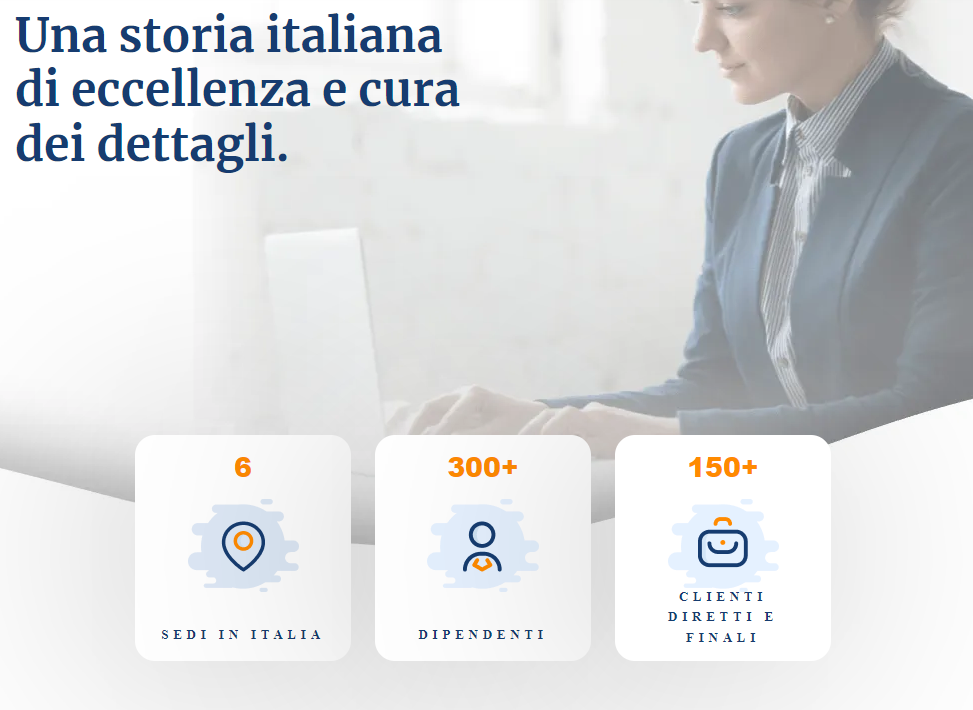
\includegraphics[scale=0.50]{azienda.png}
    \caption{Punti di forza di SyncLab}
\end{figure}
\subsection{Prodotti}
Come accennato, SyncLab opera nel settore IT e i suoi prodotti nascono dalle competenze acquisite e maturate durante le loro 20 anni di collaborazioni. I prodotti coprono vari ambiti come quelli delle telecomunicazioni, utilities, finanza e salute.
\begin{figure}[H]
    \centering
    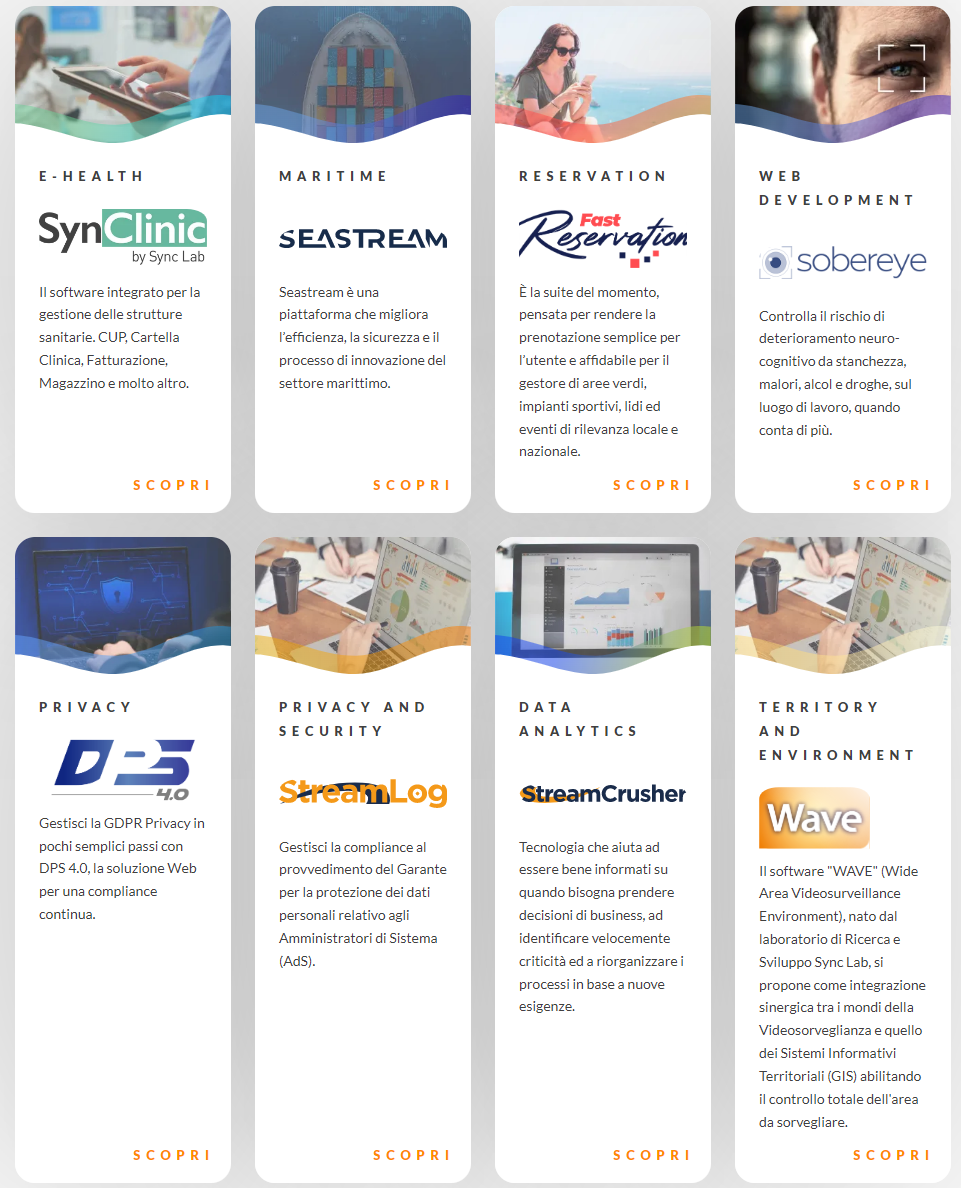
\includegraphics[width=0.55\textwidth]{prodotti.png}
    \caption{I vari prodotti di SyncLab}
\end{figure}
\begin{itemize}
    \item \textbf{SynClinic:} software integrato per la gestione delle strutture sanitarie, come il sistema di cartella clinica digitale, il servizio di fatturazione, la gestione informatizzata dei farmaci, gli strumenti nativi di gestione amministrativa e tanto altro.
    \item \textbf{SEASTREAM:} una piattaforma nata per migliorare e potenziare le attività di business nel settore armatoriali e di altri operatori del mercato marittimo.
    \item \textbf{FastReservation:} applicazione realizzata per rendere il sistema di prenotazione più facile e affidabile per gli utenti.
    \item \textbf{Sobereye:} soluzione per la sicurezza proattiva per la prevenzione degli incidenti nei settori di trasporti, estrazione, costruzioni e industrale.
    \item \textbf{DPS 4.0:} applicativo che permette di gestire la GDPR Privacy Policy. L'applicativo, tramite una guida semplice sviluppata dagli ingegneri esperti nell'ambito dell'user experience, offre la possibilità di modificare ed aggiornare i documenti sulla privacy con il minimo sforzo.
    \item \textbf{StreamLog:} soluzione per la protezione dei dati personali relativo agli amministratori di sistema, offre la possibilità di effettuare il controllo degli accessi degli utenti ai sistemi in modo semplice ed efficace.
    \item \textbf{StreamCrusher:} tecnologia che serve per aiutare a prendere decisioni di business, indentificando velocemente i punti critici e riformando i processi in base alle nuove esigenze.
    \item \textbf{Wave:} software nato per i sistemi di videosorverglianza, con l'obiettivo di avere una maggiore copertura territoriale col minor numero di telecamere installate e possibilmente utilizzare il minor numero possibile di risorse.
\end{itemize}

\section{Introduzione al progetto}
Lo scopo dello stage quello di realizzare una web-app per la gestione delle ordinazioni dei piatti di un ristorante sushi "all you can eat" con tale formula i ristoranti offrono la possibilità di ordinare senza limiti ad un prezzo fisso. Quindi i consumi dei clienti in questi locali è maggiore rispetto ai ristoranti tradizionali, perché con la formula "all-you-can-eat" spesso i clienti mangiano oltre il loro livello di sazietà, oltre a questo il menù contiene centinaia di piatti diversi, di seguito comporterà un elevato numero di ordinazioni da gestire creando così il problema di capire poi chi ha ordinato un specifico piatto nel momento della consegna.

\section{La soluzione individuata}
SyncLab ha deciso di risolvere questo problema tramite SushiLab, una web-app che offre la possibilità agli utenti di ordinare i piatti e tracciare tutte le ordinazioni.\\ 
Un'utente può inoltre registrarsi alla piattaforma per salvare dei piatti nella propria lista dei preferiti, aggiungere ingredienti alla propria blacklist e recensire un piatto.\\
SushiLab è composta da due parti, la parte \gls{frontendg} e la parte \gls{backendg}. Il \gls{backendg} deve essere implementato tramite Java utilizzando il framework \gls{Springg} e ha il ruolo pricipale di un web server, che deve comunicare con il data-base, dove vengono salvati tutte le informazioni dei piatti e tutti gli ordini effettuati dai clienti.
La parte di front-end è invece realizzato in Javascript, utilizzando il framework Angular. La comunicazione tra le due parti della web-app avviene tramite le chiamate \gls{restg} fornite dal \gls{backendg}.
Per ciascuna parte dell'applicazione è stata affidata a più persone. Discutendo con il tutor aziendale, Fabio Pallaro, abbiamo individuato i principali obiettivi per realizzare la web-app ed a me è stato assegnato il compito di sviluppare la visuale dell'applicazione. 
Si è deciso di realizzare una web-app perché non c'è la necessità di scaricare ed installare applicativo, così riducendo il tempo delle ordinazioni dei clienti.

\begin{figure}[H]
    \centering
    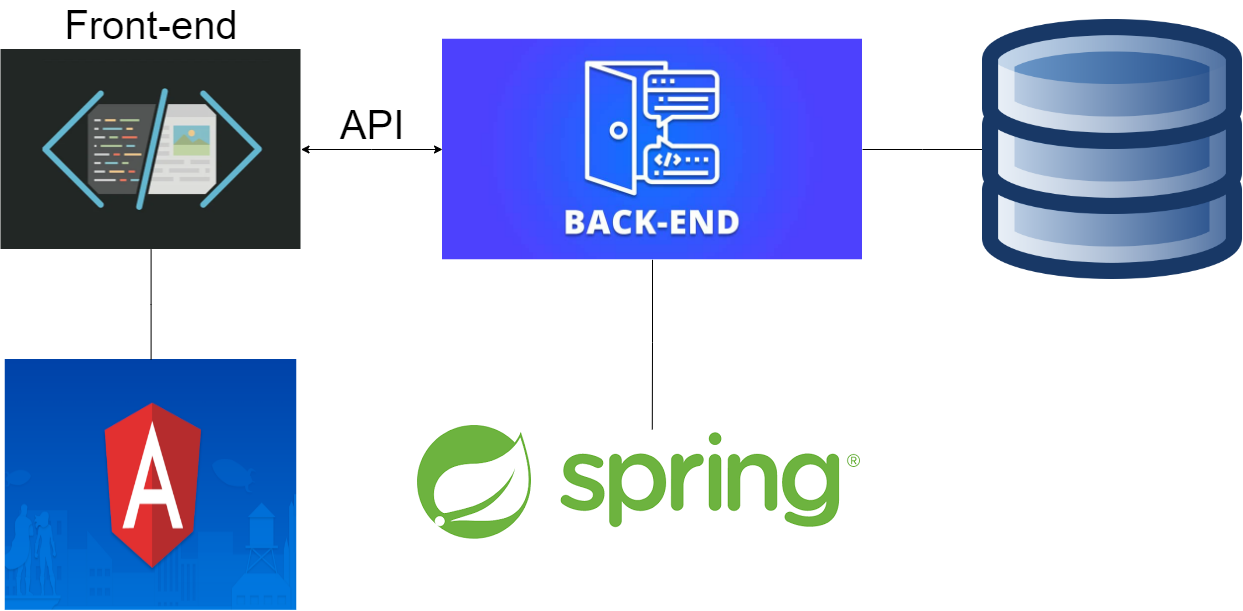
\includegraphics[scale=0.27]{diagramma.png}
    \caption{Diagramma dei componenti per la web-app}
\end{figure}
%**************************************************************


%**************************************************************
\section{Organizzazione del testo}

\begin{description}
    \item[{\hyperref[cap:il progetto di stage]{Il secondo capitolo}}] descrive in dettaglio la pianificazione e gli obiettivi dello stage.
    
    \item[{\hyperref[cap:analisi dei requisiti]{Il terzo capitolo}}] descrive l'analisi dei requisiti della web-app, vengono discussi tutti i casi d'uso e i requisiti da rispettare.
    
    \item[{\hyperref[cap:progettazione e codifica]{Il quarto capitolo}}] approfondisce la progettazione e codifica, elencando i vari componenti e descrivendo le loro funzionalità.
    
    % \item[{\hyperref[cap:progettazione-codifica]{Il quinto capitolo}}] approfondisce ...
    
    \item[{\hyperref[cap:verifica]{Il quinto capitolo}}] approfondisce la fase di verifica e validazione della web-app.
    
    \item[{\hyperref[cap:conclusioni]{Il sesto capitolo}}] descrive le conclusioni dell'intero progetto, parlando del prodotto finale e le competenze acquisite durante lo stage.
\end{description}
Riguardo la stesura del testo, relativamente al documento sono state adottate le seguenti convenzioni tipografiche:
\begin{itemize}
	\item gli acronimi, le abbreviazioni e i termini ambigui o di uso non comune menzionati vengono definiti nel glossario, situato alla fine del presente documento;
	\item per la prima occorrenza dei termini riportati nel glossario viene utilizzata la seguente nomenclatura: \emph{parola}\glsfirstoccur;
	\item i termini in lingua straniera o facenti parti del gergo tecnico sono evidenziati con il carattere \emph{corsivo}.
\end{itemize}             % Introduzione
% !TEX encoding = UTF-8
% !TEX TS-program = pdflatex
% !TEX root = ../tesi.tex

%**************************************************************
\chapter{Il progetto di stage}
\label{cap:il progetto di stage}
%**************************************************************

\intro{In questo capitolo, viene descritta la pianificazione e gli obiettivi dello stage. Infine vengono elencati gli strumenti utilizzati durante lo svolgimento dello stage.}\\

%**************************************************************


\section{Pianificazione del lavoro}
\subsection*{Pianificazione settimanale}
\begin{itemize}
    \item Prima Settimana (40 ore)
    \begin{itemize}
        \item Incontro con persone coinvolte nel progetto per discutere i requisiti e le richieste relativamente
        al sistema da sviluppare;
        \item Presentazione strumenti di lavoro per la condivisione del materiale di studio e per la gestione
        dell'avanzamento;
        \item Condivisione scaletta di argomenti;
        \item Ripasso del linguaggio Java SE;
        \item Ripasso concetti Web (Servlet, servizi REST, Json ecc.).
    \end{itemize}
    \item Seconda Settimana (40 ore)
        \begin{itemize}
            \item Studio principi generali di Spring Core (IOC, Dependency Injection);
            \item Studio SpringBoot;
            \item Studio Spring Data/DataRest.
        \end{itemize}
    \item Terza Settimana (40 ore)
        \begin{itemize}
            \item Ripasso linguaggio Javascript;
            \item Studio del linguaggio TypeScript.
        \end{itemize}
    \item Quarta Settimana (40 ore)
        \begin{itemize}
            \item Studio piattaforma NodeJS e AngularCLI;
            \item Studio framework Angular.
        \end{itemize}
    \item Quinta Settimana (40 ore)
        \begin{itemize}
        \item Analisi e studio del progetto SushiLab;
        \item Progettazione ed implementazione della nuova maschera di accesso.
        \end{itemize}
    \item Sesta Settimana (40 ore)
    \begin{itemize}
        \item Progettazione ed implementazione nuova maschera "Inserimento Ordine e gestione del tavolo".
    \end{itemize}
    \item Settima Settimana (40 ore)
    \begin{itemize}
        \item Progettazione ed implementazione nuova maschera "Merge Ordini e Visualizzazione Ordine unico".
    \end{itemize}
    \item Ottava Settimana - Conclusione (40 ore)
    \begin{itemize}
        \item Verifica del funzionamento della web-app;
        \item Validazione della web-app;
        \item Termine integrazioni e collaudo finale.
    \end{itemize}
\end{itemize}

\section{Obiettivi richiesti}
\subsection{Notazione}
Si farà riferimento ai requisiti secondo le seguenti notazioni:
\begin{itemize}
    \item O per i requisiti obbligatori, vincolanti in quanto obiettivo primario richiesto dal committente;
    \item D per i requisiti desiderabili, non vincolanti o strettamente necessari, ma dal riconoscibile valore
    aggiunto;
    \item F per i requisiti facoltativi, rappresentanti valore aggiunto non strettamente competitivo.
\end{itemize}
Le sigle precedentemente indicate saranno seguite da una coppia sequenziale di numeri, identificativo del
requisito.
\subsection{Obiettivi fissati}
Si prevede lo svolgimento dei seguenti obiettivi:
\begin{itemize}
    \item Obbligatori:
    \begin{itemize}
        \item O01: Acquisizione competenze sulle tematiche sopra descritte;
        \item O02: Capacità di raggiungere gli obiettivi richiesti in autonomia seguendo il cronoprogramma;
        \item O03: Portare a termine le implementazioni previste con una percentuale di superamento pari al 80\%.
    \end{itemize}
    \item Desiderabili:
     \begin{itemize}
        \item D01: Portare a termine le implementazioni previste con una percentuale di superamento pari al 100\%.
     \end{itemize}
     \item Facoltativi:
     \begin{itemize}
        \item F01: Apportare un valore aggiunto al gruppo di lavoro durante le fasi di progettazione delle interfacce.
     \end{itemize}
\end{itemize}


\section{Modalità di lavoro}
L'azienda utilizza lo sviluppo agile del software. La modalità agile aiuta a ridurre il rischio di fallimento sviluppando il software in finestre di tempo limitate, chiamate iterazioni, che in genere durano qualche settimana. Ogni iterazione è un piccolo progetto a sé stante e deve contenere tutto ciò che è necessario per rilasciare un piccolo incremento nelle funzionalità del software: pianificazione, analisi dei requisiti, progettazione, implementazione, test e documentazione. Ogni settimana viene effettuato un incontro con il tutor aziendale per discutere dei problemi trovati durante lo sviluppo e fare il punto della situazione del progetto.

\section{Strumenti utilizzati}
\subsection{Comunicazione:}
Per avere una buona comunicazione con l'azienda si è deciso di utilizzare:
\subsubsection{Discord:}
Una piattaforma di \gls{voipg}, messaggistica istantanea e distribuzione digitale. Su discord gli utenti comunicano con chiamate vocali, video chiamate ed è anche possibile condividere lo schermo.
\begin{figure}[H]
    \centering
    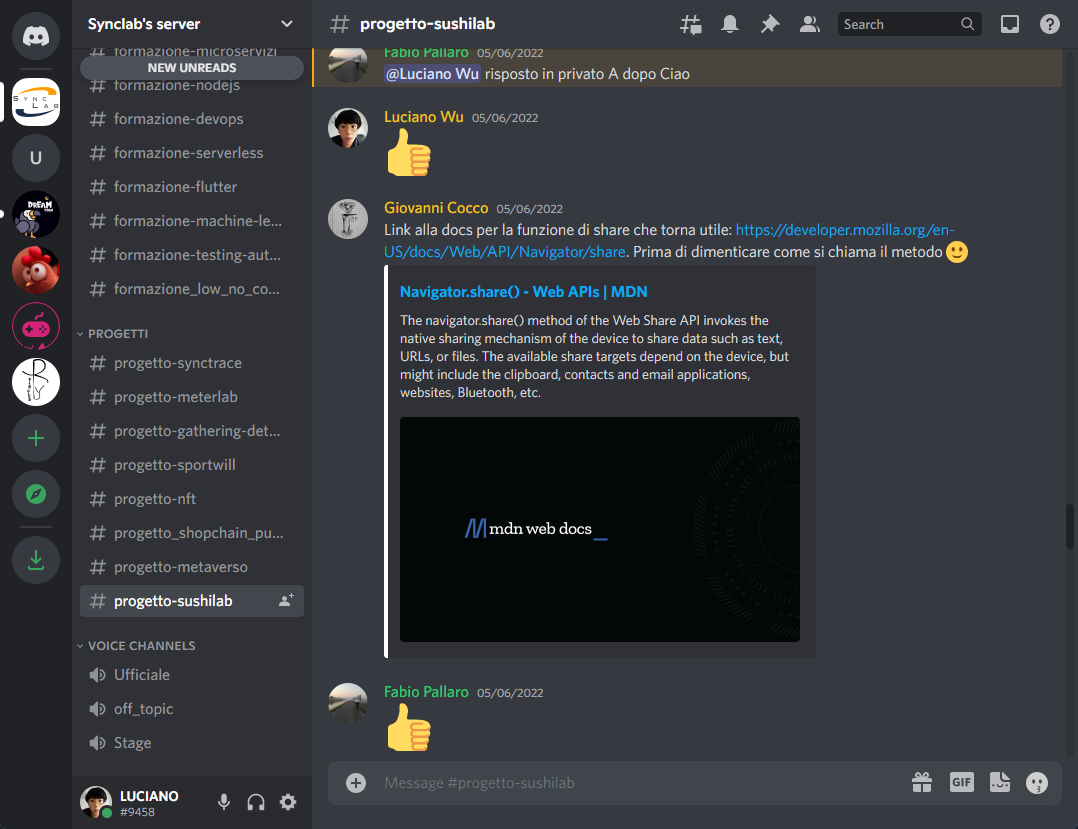
\includegraphics[scale=0.3]{discord.png}
    \caption{Canale SyncLab su Discord}
\end{figure}
\subsubsection{Trello:}
Un software gestionale in stile Kanban, in cui è possibile pianificare il progetto, condividere lo stato di svolgimento di una card con altri collaboratori, spostare varie card tra le liste e assegnarle ad un utente.
\begin{figure}[H]
    \centering
    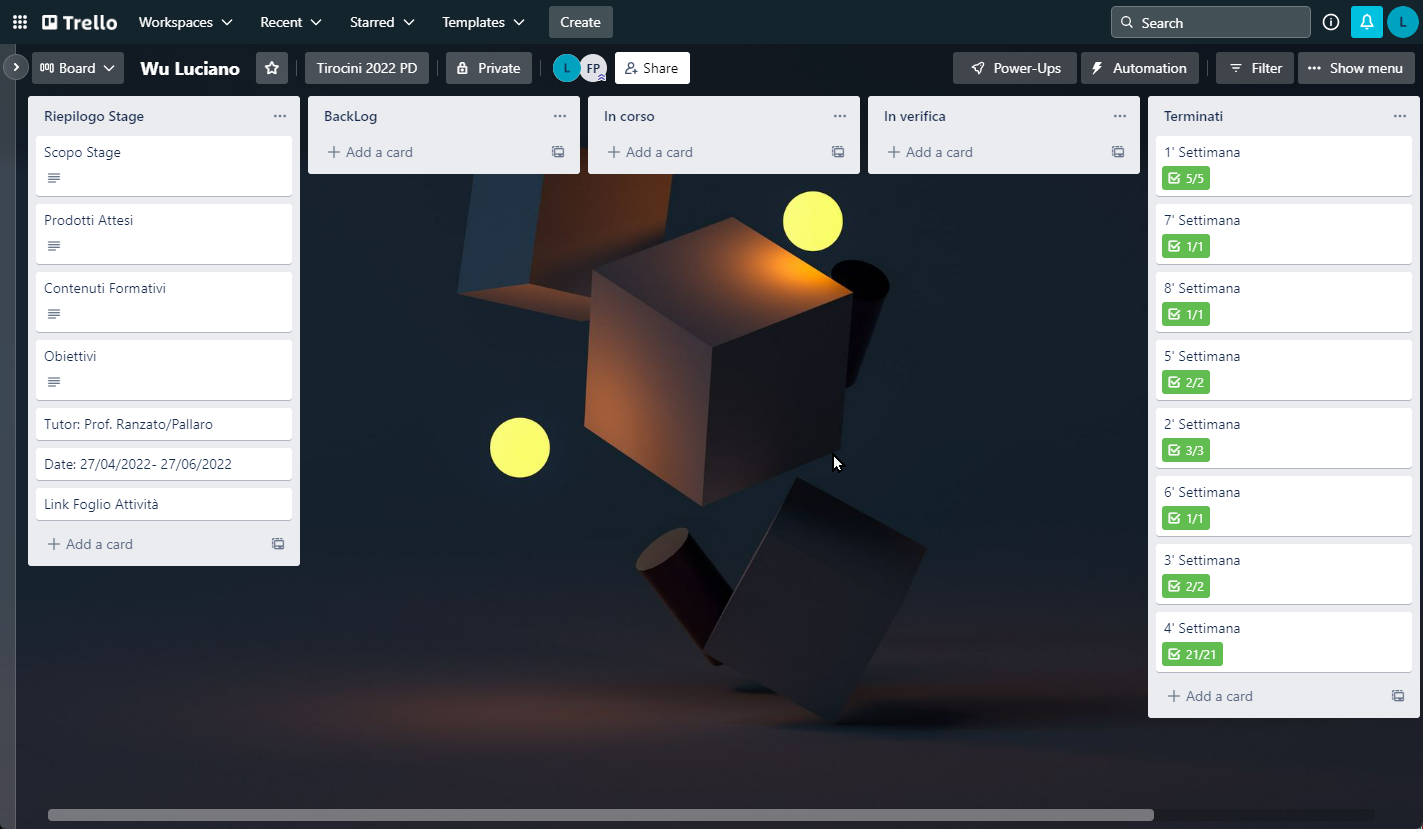
\includegraphics[scale=0.3]{trello.png}
    \caption{Board di Trello per il progetto sushi-lab}
\end{figure}
\subsubsection{Google Sheets:}
Una web-app che fornisce tutte le funzionalità di un foglio elettronico, lo abbiamo utilizzato come un diario giornaliero, dove vengono descritti i compiti svolti durante una certa giornata.
\begin{figure}[H]
    \centering
    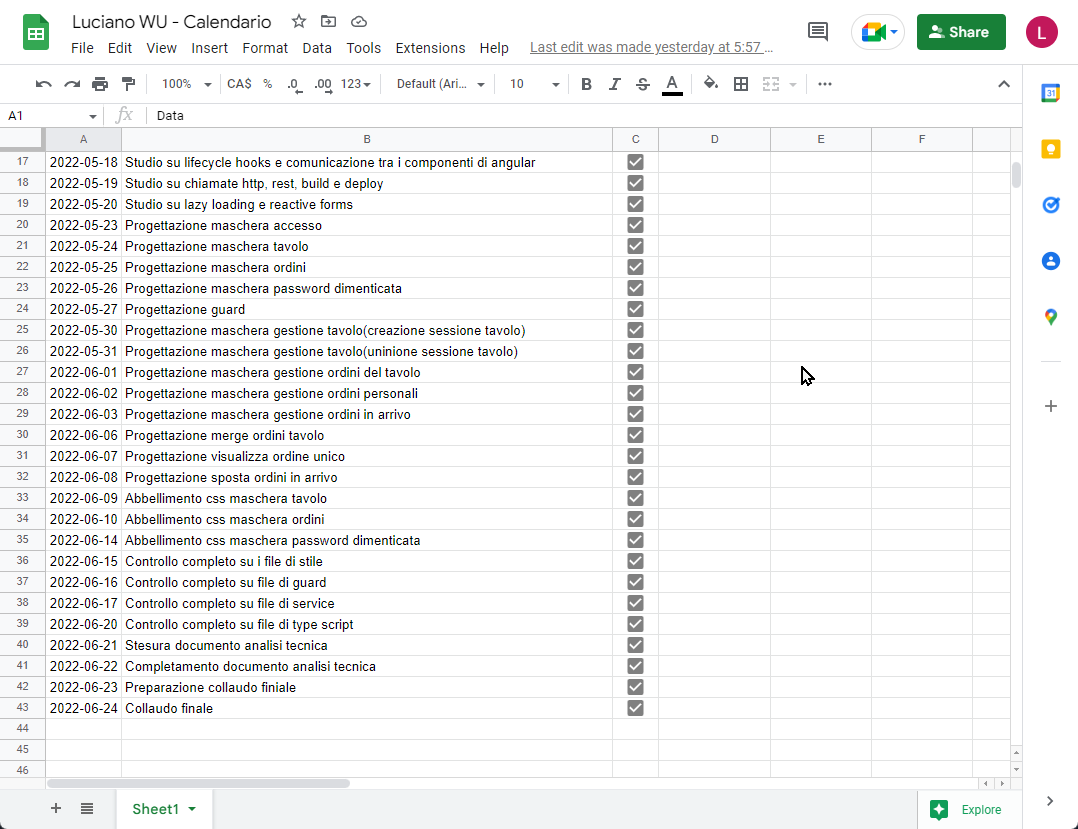
\includegraphics[scale=0.3]{googlesheet.png}
    \caption{Calendario personale per il progetto sushi-lab}
\end{figure}
\subsubsection{Google Meet:}
Un software nato per le videochiamate sviluppato da Google, in cui è possibile mandare messaggi, condividere lo schermo e l'audio contemporaneamente, lo abbiamo utilizzato per alcuni incontri con alcuni collaboratori esterni per analisi dei requisiti.
\subsection{Sviluppo:}
Per avere una buona efficienza per lo sviluppo della web-app vengono utilizzati gli strumenti più popolari per lo sviluppo, che sono:
\subsubsection{GitHub:}
Servizio di hosting per lo sviluppo software, è implementato insieme con lo strumento di controllo di versione distribuito \gls{Gitg}, nel mio caso è stato utilizzato per condividere e tracciare i file con gli altri collaboratori del progetto.
\begin{figure}[H]
    \centering
    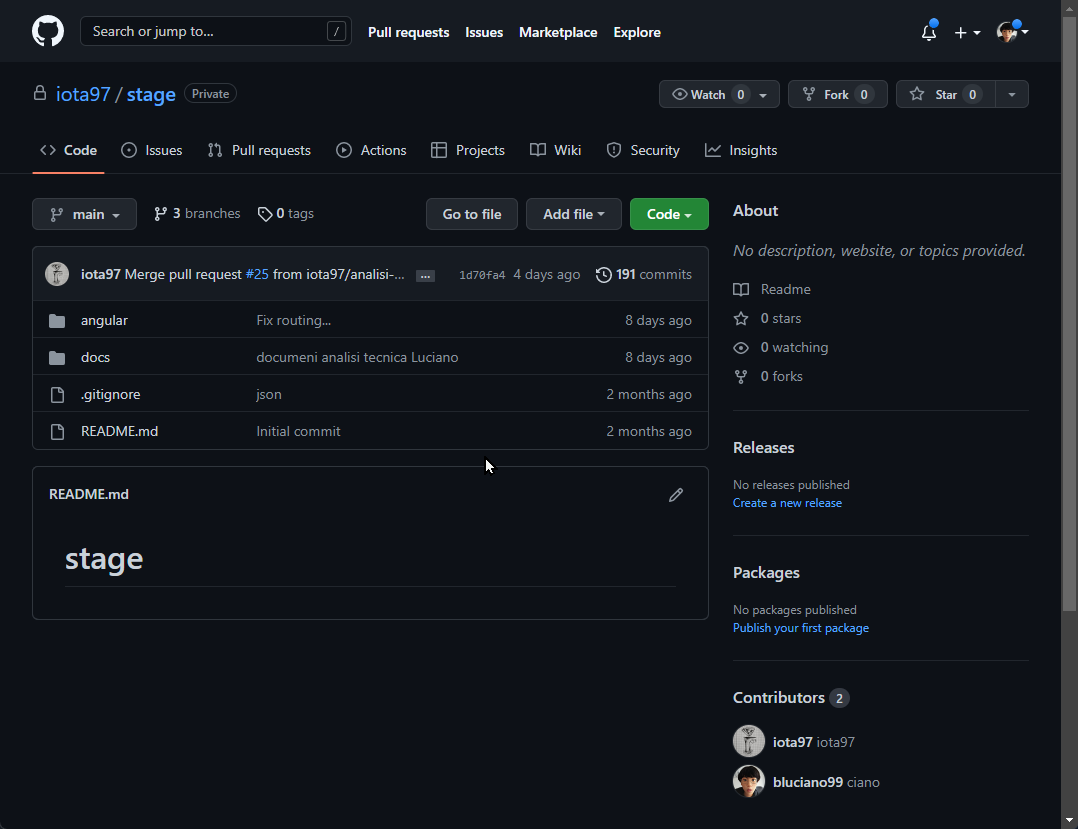
\includegraphics[scale=0.3]{github.png}
    \caption{Repo su GitHub per il progetto sushi-lab}
\end{figure}
\subsubsection{Visual Studio Code:}
Un editor sviluppato da Microsoft. Contiene tutte le funzionalità di un editor ed è completamente gratuito. Le principali funzionalità utilizzate per il progetto sono:
\begin{itemize}
    \item Le estensioni per il codice html, css e TypeScript;
    \item Il source control di Git integrato con Visual Studio Code;
    \item La funzione search con la quale è possibile ricercare un termine dentro tutti i file e farne la sostituzione.
\end{itemize}
\begin{figure}[H]
    \centering
    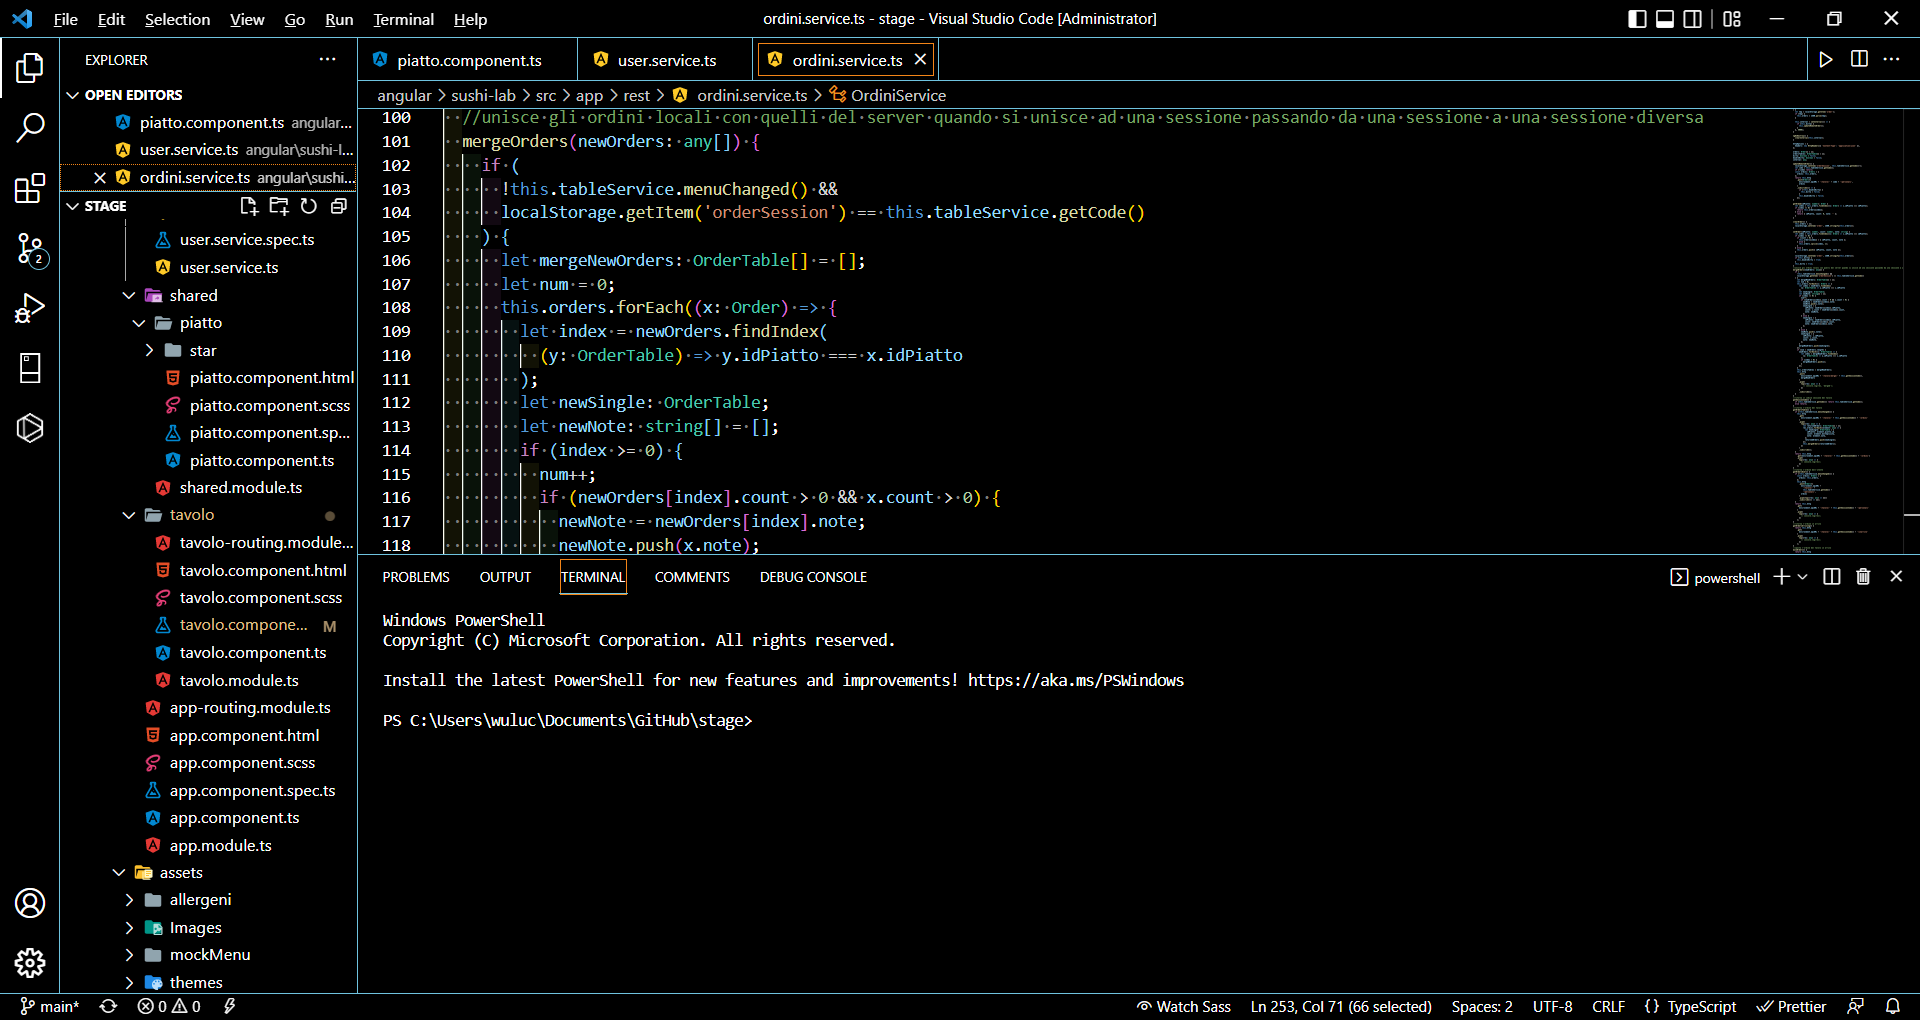
\includegraphics[scale=0.35]{vscode.png}
    \caption{Interfaccia di Visual Studio Code}
\end{figure}
\subsubsection{Google Chrome:}
Un browser web sviluppato da Google. È il browser più popolare al mondo grazie alla sua buona stabilità ed elevata velocità. La principale funzionalità utilizzata di Chrome durante lo sviluppo sono gli strumenti per sviluppatori, che permette di vedere tutti i dati di uno specifico elemento HTML presente nella pagina, in più è possibile vedere tutti i dati salvati in locale della pagina.
\begin{figure}[H]
    \centering
    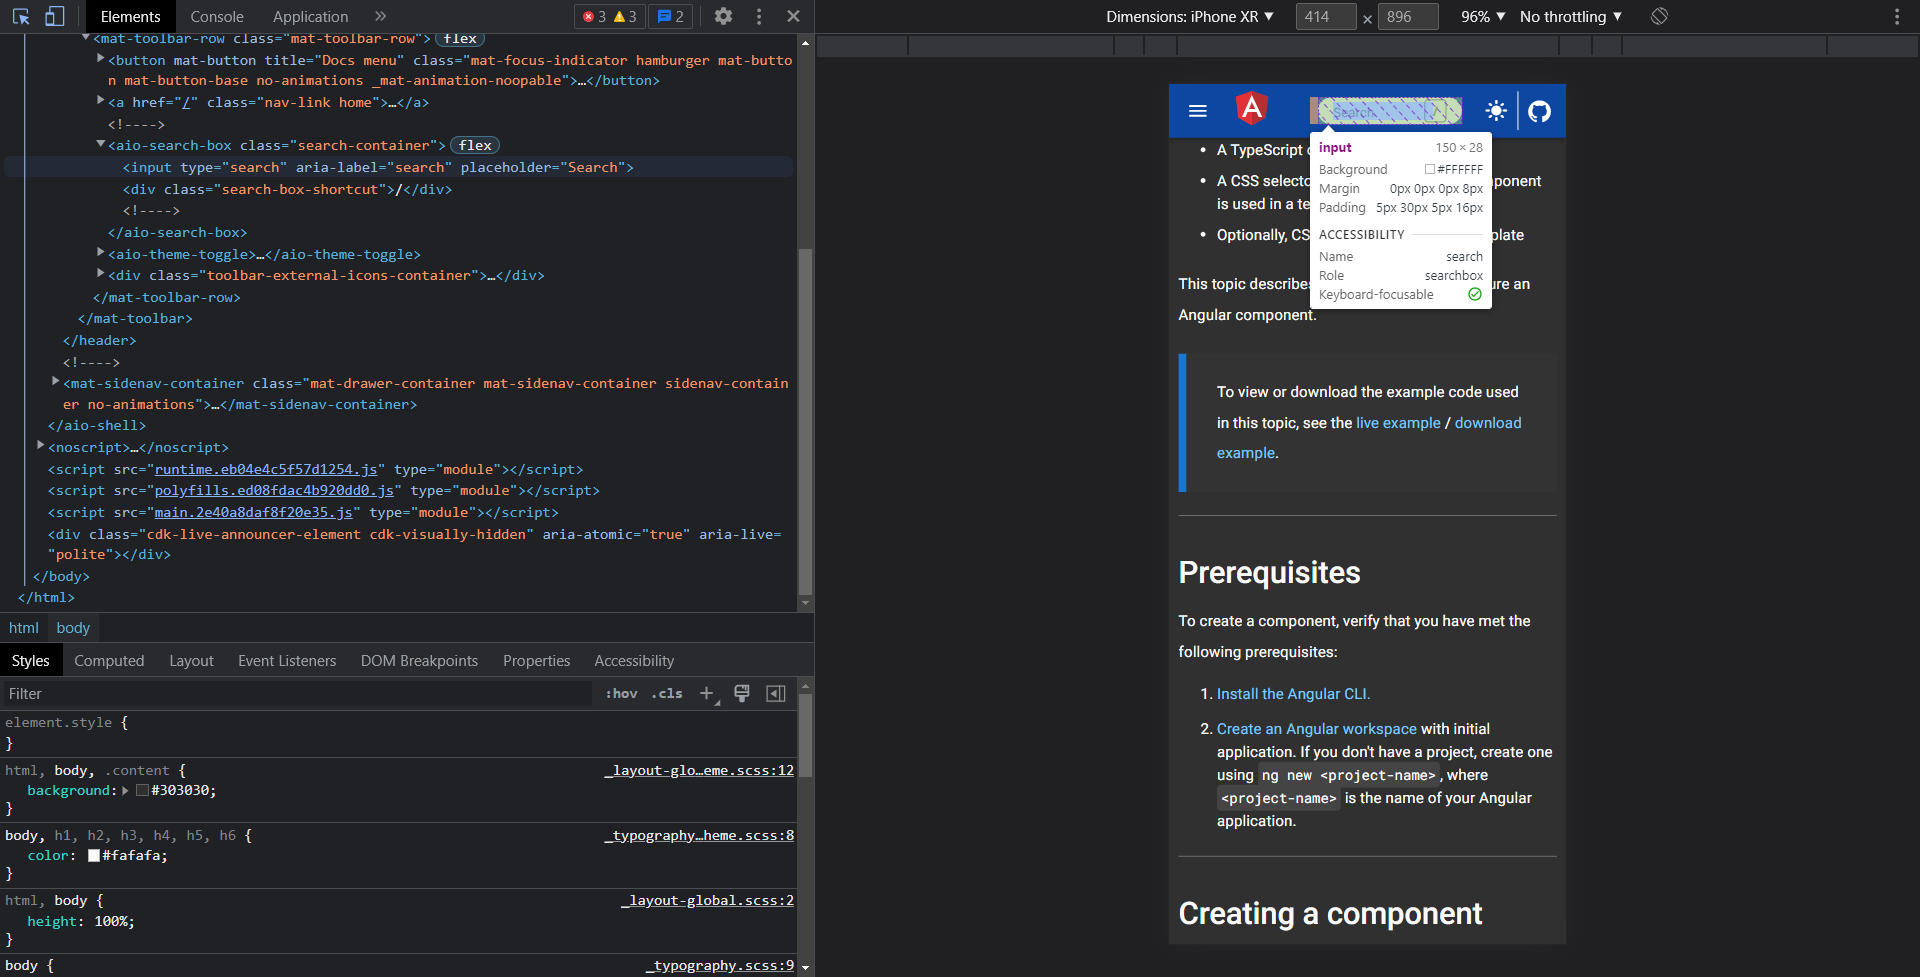
\includegraphics[scale=0.3]{chrome.png}
    \caption{Interfaccia con lo strumento ispeziona di Google Chrome}
\end{figure}
% \begin{center}
    
%     \begin{tabular}{ |p{3cm}|p{3cm}|p{3cm}|  }
%         \hline
%         \multicolumn{3}{|c|}{Country List} \\
%         \hline
%         Country Name or Area Name& ISO ALPHA 2 Code &ISO ALPHA 3 \\
%         \hline
%         Afghanistan & AF &AFG \\
%         Aland Islands & AX   & ALA \\
%         Albania &AL & ALB \\
%         Algeria    &DZ & DZA \\
%         American Samoa & AS & ASM \\
% Andorra & AD & AND   \\
% Angola & AO & AGO \\
% \hline
% \end{tabular}
% \end{center}             % Processi
% !TEX encoding = UTF-8
% !TEX TS-program = pdflatex
% !TEX root = ../tesi.tex

%**************************************************************
\chapter{Analisi dei requisiti}
\label{cap:analisi dei requisiti}
%**************************************************************

\intro{In questo capitolo vengono trattati le analisi dei requisiti del modulo di front-end della web-app, con i vari casi d'uso ed elenco dei requisiti.}\\

%**************************************************************
\section{Descrizione generale}
\subsection{interfacce della web-app}
\subsubsection{Interfaccia menù}
L'utente può visualizzare il menù di un ristorante dopo aver scansionato il QR-code di un ristorante presente sul tavolo. Il menù è composto da un insieme di categorie, in cui ci sono tutti i piatti appartenenti a quella categoria. I piatti sono ordinati in base al suo id che è un numero univoco dentro ogni menù.
\subsubsection{Interfaccia lista ordini}
L'utente può vedere i piatti ordinati del suo tavolo di appartenenza, dove ci sono anche i piatti ordinati dalle altre persone del tavolo, inoltre può vedere i suoi piatti personali e i piatti in arrivo.
\subsubsection{Interfaccia gestione tavolo}
In questa maschera utente può creare una sessione di tavolo se non appartiene ad nessuna sessione, altrimenti può visuale il suo QR-code in modo da fare entrare gli altri nella sua sessione di tavolo.
\subsubsection{Interfaccia area personale}
Qui l'utente può effetture la login, di seguito se ha degli allergeni potrà inserire degli ingredienti nella blacklist\gl{} in modo tale di non visualizzare i piatti contenenti quegli ingredienti nella sezione menù.
\subsection{Caratteristiche degli Utenti}
In questa sezione vengono descritti tutte le Caratteristiche degli utenti che possono utilizzare la web-app.
\subsubsection{Utente non autenticato}
Con il termine utente non autenticato ci si riferisce ad una qualsiasi persona non autenticata nel sistema, che può sfruttare le funzionalità di base offerte dalla piattaforma, ossia:
\begin{itemize}
    \item Visualizzare il menù del ristorante;
    \item Visualizzare i singoli piatti in modalità dettaglio;
    \item Creare una sessione di tavolo;
    \item Unire ad una sessione di tavolo già esistente;
    \item Uscire dalla sessione di tavolo;
    \item Aggiungere piatti negli ordini;
    \item Aggiungere note ai piatti ordinati;
    \item Spostare ordini in arrivo;
    \item Marcare i piatti in arrivo come arrivato;
    \item Registrare nella piattaforma;
    \item Effettuare la login.
\end{itemize}
\subsubsection{Utente autenticato}
Invece, con il termine “utente autenticato” ci si riferisce ad una persona registrata nel database e che ha effettuato l'accesso nella piattaforma, la quale, oltre a sfruttare le funzionalità dell'utente non autenticato, può anche:
\begin{itemize}
    \item Aggiungere piatti nei preferiti;
    \item Rimuovere piatti dai preferiti;
    \item Dare un recensione ad un piatto;
    \item Aggiungere ingredienti non voluti;
    \item Rimuovere gli ingredienti non voluti;
    \item Effettuare logout.
\end{itemize}
%**************************************************************
\subsection{Tecnologie utilizzate}
Per sviluppare la piattaforma verranno utilizzare le seguenti tecnologie:
\begin{itemize}
    \item HTML5\gl{}: per creare la struttura dell'interfaccia untente;
    \item CSS3\gl{}: per lo stile dell'interfaccia, viene utilizzato la sintassi SCSS;
    \item Stoplight\gl{}: per simulare le chiamate Rest API;
    \item Angular\gl{}: per la creazione dell'interfaccia utente.
\end{itemize}
\subsection{Descrizione delle tecnologie}
\subsubsection{HTML5}
L'HyperText Markup Language, noto come HTML, è un linguaggio di markup più popolare, utilizzato per progettare le strutture dei siti web. Viene utilizzato da Angular per creare la struttura iniziale per le varie interfacce, poi queste strutture vengono modificate da Angular per generare la pagina dinamicamente. 
\subsubsection{CSS3}
Il CSS, sigla di Cascading Style Sheets, è il linguaggio utilizzato per modificare il layout delle pagine web, le regole vengono applicate nel ordine in cui vengono scritte. Per il progetto è stato utilizzato una sua estensione SCSS, la quale è compatibile con tutte le versioni di CSS. Tramite la SCSS è possibile dichiarare le regole CSS in blocchi quindi ci aiuta a scrivere regole CSS in più velocemente e comprensibile.
\subsubsection{TypeScript}
TypeScript è un linguaggio di programmazione open source sviluppato da Microsoft, che estende il classico JavaScript quindi qualsiasi codice scritto in JavaScript è anche eseguibile con TypeScript direttamente senza nessuna modifica. TypeScript rende molto più flessibile e flessibile JavaScript aggiungendo la firma dei metodi, classi, tipi di dato e tanto altro, grazie a queste caratteristiche utilizzando TypeScript ci ganrantisce controlli automatici, rilevando in automatico i bug prima della compilazione.
\subsubsection{Angular}
Angular è un framework open source per sviluppare applicazioni web, permette di dividere l'applicazione in più componenti, grazie a questo è possibile riutilizzare lo stesso modulo in più parti della web-app, oltre a questo garantisce una maggiore manutenibilità e espandibilità.
\subsubsection{Stoplight}
Stoplight è una piattaforma che offre la possibilità di progettare le API velocemente, grazie alla sua interfaccia user friendly\gl{}. Offre un buon spazio per collabolare con gli altri, condividendo tutte le API con le sue descrizioni e risposte in modo chiaro.
\section{Casi D'uso}
\subsection{Introduzione }
In questa sezione verranno presentati i casi d'uso individuati durante la fase di analisi dei requisiti, i quali fanno riferimento a tutte le funzionalità che la web-app SushiLab dovrà offrire ad ogni utente che vorrà interfacciarsi con essa.
\subsection{Attori primari}
\begin{itemize}
    \item Utente non Autenticato: utente che non ha ancora effettuato la fase di autenticazione sulla piattaforma. Può essere in possesso o meno delle credenziali per l'autenticazione. Avrà funzionalità limitate rispetto ad un utente autenticato;
    \item Utente Autenticato: utente che ha effettuato l'autenticazione alla piattaforma tramite le proprie credenziali. Ha accesso ad ogni funzionalità messa a disposizione dalla piattaforma;
    \item  Utente Generico: può essere sia un utente autenticato che un utente non autenticato.
\end{itemize}
\subsection{Utente generico}
\subsection{UC1 - Visualizza menù}
\begin{figure}[H]
    \centering
    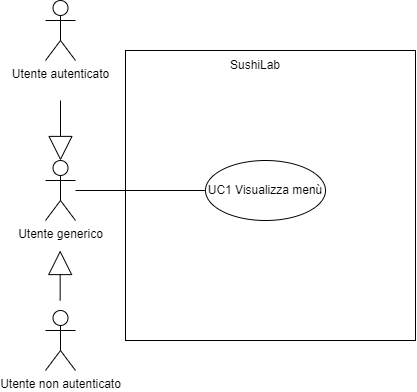
\includegraphics[scale=0.5]{usecase/tesi-uc1.drawio.png}
    \caption{Use Case - UC 1}
\end{figure}
\begin{itemize}
    \item \textbf{Descrizione:} L'utente visualizza il menù del ristorante.
    \item \textbf{Attore Primario:} Untente generico.
    \item \textbf{Precondizione:} L'utente si trova dentro la web-app sushiLab.
    \item \textbf{Postcondizione:} Viene visualizzato il menù del ristorante.
    \item \textbf{Scenrio principale:}
    \begin{itemize}
        \item L'utente si trova dentro il sistema;
        \item L'utente clicca sul bottone menù.
    \end{itemize}
\end{itemize}
\subsection{UC1.1 - Visualizza categorie}
\begin{figure}[H]
    \centering
    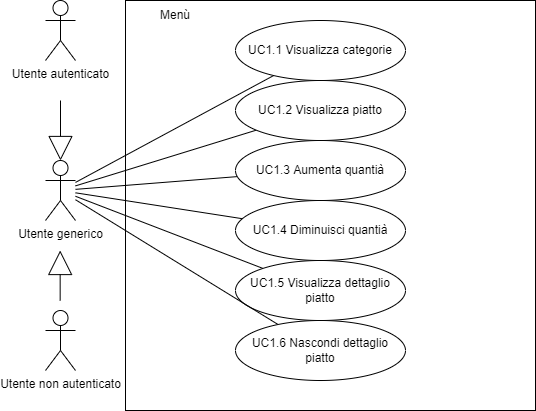
\includegraphics[scale=0.5]{usecase/tesi-uc11.drawio.png}
    \caption{Use Case - UC 1.1, UC 1.2, UC 1.3, UC 1.4, UC 1.5, UC 1.6}
\end{figure}
\begin{itemize}
    \item \textbf{Descrizione:} L'utente visualizza le categorie del menù.
    \item \textbf{Attore Primario:} Untente generico.
    \item \textbf{Precondizione:} L'utente si trova dentro la sezione menù.
    \item \textbf{Postcondizione:} Viene visualizzato i nomi delle categorie.
    \item \textbf{Scenrio principale:}
    \begin{itemize}
        \item L'utente si trova sezione menù;
        \item Viene mostrato le categorie del menù.
    \end{itemize}
\end{itemize}
\subsection{UC1.2 - Visualizza piatto}
\begin{itemize}
    \item \textbf{Descrizione:} L'utente visualizza i piatti del menù mostrando il numero, nome, prezzo, ingredienti\gl{}, allergeni, limatazioni\gl{} e la quantità. La quantità di default\gl{} è 0 che vuole dire non è stato ordinato.
    \item \textbf{Attore Primario:} Untente generico.
    \item \textbf{Precondizione:} L'utente si trova dentro la sezione menù.
    \item \textbf{Postcondizione:} Viene visualizzato i piatti del menù.
    \item \textbf{Scenrio principale:}  
    \begin{itemize}
        \item L'utente si trova sezione menù;
        \item Viene mostrato i piatti del menù.
    \end{itemize}
\end{itemize}
\subsection{UC1.3 - Aumenta quantità}
\begin{itemize}
    \item \textbf{Descrizione:} L'utente aumenta la quantità di un piatto nel menù.
    \item \textbf{Attore Primario:} Untente generico.
    \item \textbf{Precondizione:} L'utente si trova dentro la sezione menù.
    \item \textbf{Postcondizione:} Viene aggiunto il piatto specifico con la quantità aggiornata negli ordini.
    \item \textbf{Scenrio principale:}
    \begin{itemize}
        \item L'utente si trova sezione menù;
        \item L'utente clicca sul bottone + di un piatto;
        \item Viene aggiunto il piatto negli ordini.
    \end{itemize}
    \item \textbf{Scenrio alternativo:}
    \begin{itemize}
        \item L'utente si trova sezione menù;
        \item L'utente clicca sul bottone + di un piatto che è già presente negli ordini;
        \item Viene aumentato la quantità del piatto negli ordini.
    \end{itemize}
\end{itemize}
\subsection{UC1.4 - Diminuisci quantità}
\begin{itemize}
    \item \textbf{Descrizione:} L'utente dimiuisce la quantità di un piatto nel menù.
    \item \textbf{Attore Primario:} Untente generico.
    \item \textbf{Precondizione:} L'utente si trova dentro la sezione menù.
    \item \textbf{Postcondizione:} Viene dimiuito la quantità del piatto specifico negli ordini.
    \item \textbf{Scenrio principale:}
    \begin{itemize}
        \item L'utente si trova sezione menù;
        \item L'utente clicca sul bottone - di un piatto con quantità maggiore di 1;
        \item Viene diminuito la quantità del piatto negli ordini.
    \end{itemize}
    \item \textbf{Scenrio alternativo:}
    \begin{itemize}
        \item L'utente si trova sezione menù;
        \item L'utente clicca sul bottone - di un piatto con quantità uguale a 1;
        \item Viene rimosso il piatto dagli ordini.
    \end{itemize}
\end{itemize}
\subsection{UC1.5 - Visualizza dettaglio piatto}
\begin{itemize}
    \item \textbf{Descrizione:} L'utente visualizza i dettagli di un piatto nel menù, mostrando la recensione del piatto e il text-box\gl{} per inserire una nota.
    \item \textbf{Attore Primario:} Untente generico.
    \item \textbf{Precondizione:} L'utente si trova dentro la sezione menù.
    \item \textbf{Postcondizione:} Viene visualizzato i dettagli di un piatto specifico.
    \item \textbf{Scenrio principale:}  
    \begin{itemize}
        \item L'utente si trova sezione menù;
        \item L'utente clicca sul bottom mostra dettagli;
        \item Viene mostrato i dettagli di un piatto del menù.
    \end{itemize}
\end{itemize}
\subsection{UC1.6 - Nascondi dettaglio piatto}
\begin{itemize}
    \item \textbf{Descrizione:} L'utente nasconde i dettagli di un piatto specifico.
    \item \textbf{Attore Primario:} Untente generico.
    \item \textbf{Precondizione:} L'utente si trova dentro la sezione menù con un piatto in modalità dettaglio.
    \item \textbf{Postcondizione:} Viene nascosto i dettagli del piatto specifico.
    \item \textbf{Scenrio principale:}  
    \begin{itemize}
        \item L'utente si trova sezione menù;
        \item L'utente clicca sul bottom nascondi dettagli;
        \item Viene mostrato i dettagli di un piatto del menù.
    \end{itemize}
\end{itemize}
\subsection{UC2 - Gestione tavolo}
\begin{figure}[H]
    \centering
    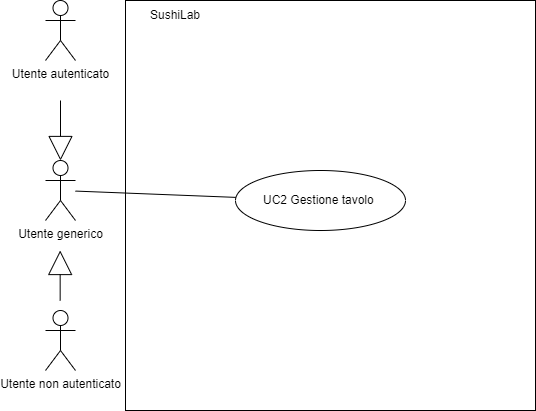
\includegraphics[scale=0.5]{usecase/tesi-uc2.drawio.png}
    \caption{Use Case - UC 2}
\end{figure}
\begin{itemize}
    \item \textbf{Descrizione:} L'utente visualizza la maschera di gestione tavolo.
    \item \textbf{Attore Primario:} Untente generico.
    \item \textbf{Precondizione:} L'utente si trova dentro la web-app sushiLab.
    \item \textbf{Postcondizione:} Viene visualizzato la maschera di gestione tavolo.
    \item \textbf{Scenrio principale:}
    \begin{itemize}
        \item L'utente si trova dentro il sistema;
        \item Viene mostrato la maschera di gestione tavolo.
    \end{itemize}
\end{itemize}
\subsection{UC2.1 - Generazione sessione tavolo}
\begin{figure}[H]
    \centering
    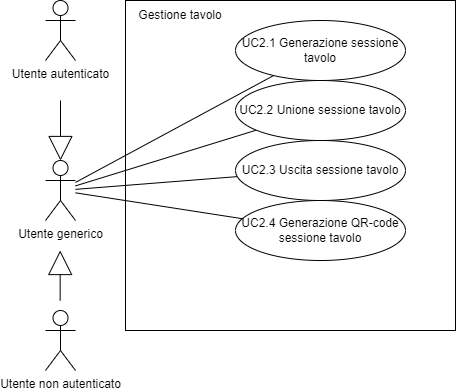
\includegraphics[scale=0.5]{usecase/tesi-uc21.drawio.png}
    \caption{Use Case - UC 2.1, UC 2.2, UC 2.3, UC 2.4}
\end{figure}
\begin{itemize}
    \item \textbf{Descrizione:} L'utente genera la sessione del tavolo.
    \item \textbf{Attore Primario:} Untente generico.
    \item \textbf{Precondizione:} L'utente si trova dentro la sezione gestione tavolo.
    \item \textbf{Postcondizione:} L'utente entra nella sessione generata del tavolo.
    \item \textbf{Scenrio principale:}
    \begin{itemize}
        \item L'utente si trova dentro la sezione gestione tavolo;
        \item L'utente clicca sul bottone crea sessione;
        \item L'utente viene inserito nella sessione creata.
    \end{itemize}
\end{itemize}
\subsection{UC2.2 - Unione sessione tavolo}
\begin{itemize}
    \item \textbf{Descrizione:} L'utente si unisce alla sessione del tavolo.
    \item \textbf{Attore Primario:} Untente generico.
    \item \textbf{Precondizione:} L'utente si trova dentro la sezione gestione tavolo.
    \item \textbf{Postcondizione:} L'utente entra nella sessione che è stata inserita.
    \item \textbf{Scenrio principale:}
    \begin{itemize}
        \item L'utente si trova dentro la sezione gestione tavolo;
        \item L'utente clicca sul bottone unisciti a una sessione;
        \item L'utente inserisce il numero della sessione;
        \item L'utente clicca sul bottone unisciti;
        \item L'utente viene inserito nella sessione.
    \end{itemize}
    \item \textbf{Scenrio alternativo:}
    \begin{itemize}
        \item L'utente si trova dentro la sezione gestione tavolo;
        \item L'utente clicca sul bottone unisciti a una sessione;
        \item L'utente inserisce il numero della sessione inesistente;
        \item L'utente clicca sul bottone unisciti;
        \item L'utente non viene inserito nella sessione.
    \end{itemize}
\end{itemize}
\subsection{UC2.3 - Uscita sessione tavolo}
\begin{itemize}
    \item \textbf{Descrizione:} L'utente esce dalla sessione del tavolo.
    \item \textbf{Attore Primario:} Untente generico.
    \item \textbf{Precondizione:} L'utente si trova dentro la sezione gestione tavolo ed è dentro ad una sessione.
    \item \textbf{Postcondizione:} L'utente esce dalla sessione generata del tavolo.
    \item \textbf{Scenrio principale:}
    \begin{itemize}
        \item L'utente si trova dentro la sezione gestione tavolo;
        \item L'utente clicca sul bottone esci dalla sessione;
        \item L'utente viene rimosso dalla sessione.
    \end{itemize}
\end{itemize}
\subsection{UC2.4 - Generazione QR-code sessione tavolo}
\begin{itemize}
    \item \textbf{Descrizione:} L'utente genera il QR-code dalla sessione del tavolo per mostrarlo agli altri, che li permetterà di unire alla sessione direttamente scansionando il QR-code.
    \item \textbf{Attore Primario:} Untente generico.
    \item \textbf{Precondizione:} L'utente si trova dentro la sezione gestione tavolo ed è dentro ad una sessione.
    \item \textbf{Postcondizione:} L'utente genera il QR-code dalla sessione del tavolo.
    \item \textbf{Scenrio principale:}
    \begin{itemize}
        \item L'utente si trova dentro la sezione gestione tavolo;
        \item L'utente genera il QR-code dalla sessione.
    \end{itemize}
\end{itemize}



\subsection{UC3 - Lista ordini}
\begin{figure}[H]
    \centering
    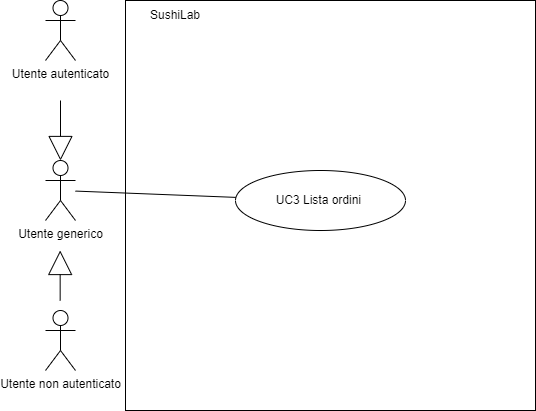
\includegraphics[scale=0.5]{usecase/tesi-uc3.drawio.png}
    \caption{Use Case - UC 3}
\end{figure}
\begin{itemize}
    \item \textbf{Descrizione:} L'utente visualizza la maschera di gestione ordini.
    \item \textbf{Attore Primario:} Untente generico.
    \item \textbf{Precondizione:} L'utente si trova dentro ad una sessione di tavolo.
    \item \textbf{Postcondizione:} Viene visualizzato la maschera di gestione ordini.
    \item \textbf{Scenrio principale:}
    \begin{itemize}
        \item L'utente si trova dentro il sistema con una sessione di tavolo attiva;
        \item Viene mostrato la maschera di gestione ordini.
    \end{itemize}
\end{itemize}
\subsection{UC3.1 - Visualizza lista ordini del tavolo}
\begin{figure}[H]
    \centering
    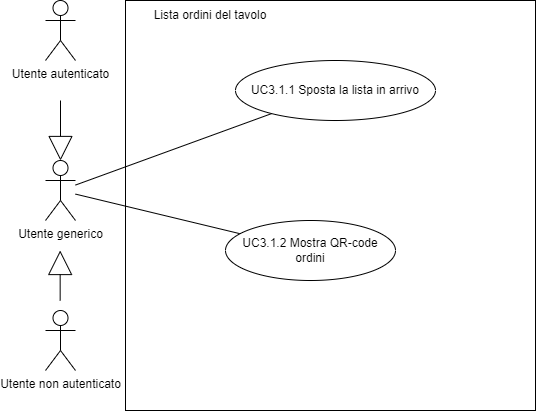
\includegraphics[scale=0.5]{usecase/tesi-uc311.drawio.png}
    \caption{Use Case - UC 3.1, UC 3.2, UC 3.3}
\end{figure}
\begin{itemize}
    \item \textbf{Descrizione:} L'utente visualizza la lista degli ordini della sessione di tavolo in cui si trova. 
    \item \textbf{Attore Primario:} Untente generico.
    \item \textbf{Precondizione:} L'utente si trova dentro la sezione lista ordini.
    \item \textbf{Postcondizione:} Viene visualizzato la lista degli ordini del tavolo.
    \item \textbf{Scenrio principale:}
    \begin{itemize}
        \item L'utente si trova dentro la sezione gestione ordini;
        \item L'utente clicca sul bottone "tavolo";
        \item Viene mostrato la lista dei piatti ordinati del tavolo.
    \end{itemize}
\end{itemize}
\subsection{UC3.2 - Visualizza lista ordini personali}
\begin{itemize}
    \item \textbf{Descrizione:} L'utente visualizzato la lista degli ordini personali.
    \item \textbf{Attore Primario:} Untente generico.
    \item \textbf{Precondizione:} L'utente si trova dentro la sezione lista ordini.
    \item \textbf{Postcondizione:} Viene visualizzato la lista degli ordini personali.
    \item \textbf{Scenrio principale:}
    \begin{itemize}
        \item L'utente si trova dentro la sezione gestione ordini;
        \item L'utente clicca sul bottone "personali";
        \item Viene mostrato la lista dei piatti ordinati dall'utente stesso.
    \end{itemize}
\end{itemize}
\subsection{UC3.3 - Visualizza lista ordini in arrivo}
\begin{itemize}
    \item \textbf{Descrizione:} L'utente visualizza la lista degli ordini in arrivo.
    \item \textbf{Attore Primario:} Untente generico.
    \item \textbf{Precondizione:} L'utente 
    \item \textbf{Postcondizione:} Viene visualizzato la lista lista degli ordini in arrivo.
    \item \textbf{Scenrio principale:}
    \begin{itemize}
        \item L'utente si trova dentro la sezione gestione ordini;
        \item L'utente clicca sul bottone "in arrivo";
        \item Viene mostrato la lista dei piatti in arrivo.
    \end{itemize}
\end{itemize}
\subsection{UC3.1.1 - Sposta la lista in arrivo}
\begin{figure}[H]
    \centering
    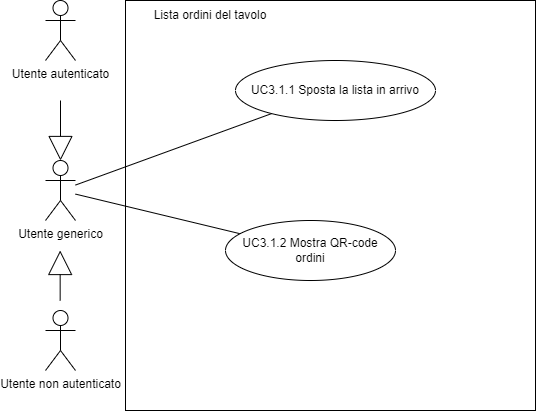
\includegraphics[scale=0.5]{usecase/tesi-uc311.drawio.png}
    \caption{Use Case - UC 3.1.1, UC 3.1.2}
\end{figure}
\begin{itemize}
    \item \textbf{Descrizione:} L'utente sposta la lista degli ordini in arrivo.
    \item \textbf{Attore Primario:} Untente generico.
    \item \textbf{Precondizione:} L'utente si trova dentro la sezione lista ordini del tavolo.
    \item \textbf{Postcondizione:} Viene spostato la lista degli ordini del tavolo in arrivo.
    \item \textbf{Scenrio principale:}
    \begin{itemize}
        \item L'utente si trova dentro la sezione gestione ordini del tavolo;
        \item L'utente clicca sul bottone sposta la lista in arrivo;
        \item Viene spostato la lista degli piatti ordinati personali in modalità dettaglio;
        \item Viene mostrato all'utente il messaggio "ordini spostati correttamente".
    \end{itemize}
\end{itemize}
\subsection{UC3.1.2 - Mostra QR-code ordini}
\begin{itemize}
    \item \textbf{Descrizione:} L'utente genera il QR-code della lista ordini per dopo mostrarlo al cameriere.
    \item \textbf{Attore Primario:} Untente generico.
    \item \textbf{Precondizione:} L'utente si trova dentro la sezione lista ordini del tavolo.
    \item \textbf{Postcondizione:} Viene mostrato il QR-code della lista degli ordini.
    \item \textbf{Scenrio principale:}
    \begin{itemize}
        \item L'utente si trova dentro la sezione gestione ordini del tavolo;
        \item L'utente clicca sul bottone QR-code;
        \item Viene generato il QR-code degli ordini.
    \end{itemize}
\end{itemize}
\subsection{UC3.2.1 - Visualizza in dettaglio lista ordini personali}
\begin{figure}[H]
    \centering
    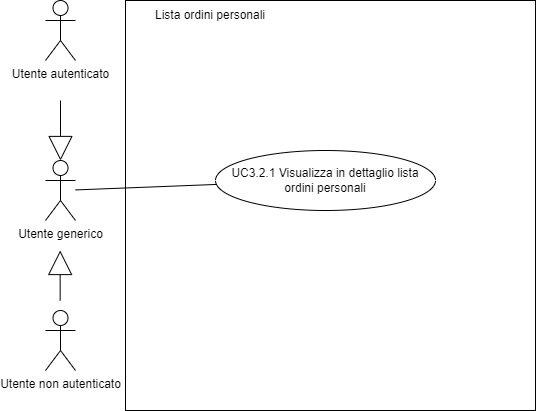
\includegraphics[scale=0.5]{usecase/tesi-uc322.drawio.png}
    \caption{Use Case - UC 3.2.1}
\end{figure}
\begin{itemize}
    \item \textbf{Descrizione:} L'utente visualizza la lista degli ordini personali in modalità dettaglio.
    \item \textbf{Attore Primario:} Untente generico.
    \item \textbf{Precondizione:} L'utente si trova dentro la sezione lista ordini personali.
    \item \textbf{Postcondizione:} Viene visualizzato la lista degli ordini personali con i piatti in modalità dettaglio.
    \item \textbf{Scenrio principale:}
    \begin{itemize}
        \item L'utente si trova dentro la sezione gestione ordini personali;
        \item L'utente clicca sul bottone "lente" con il +;
        \item Viene mostrato la lista dei piatti ordinati personali in modalità dettaglio.
    \end{itemize}
\end{itemize}
\subsection{UC3.3.1 - Ricezione piatto}
\begin{figure}[H]
    \centering
    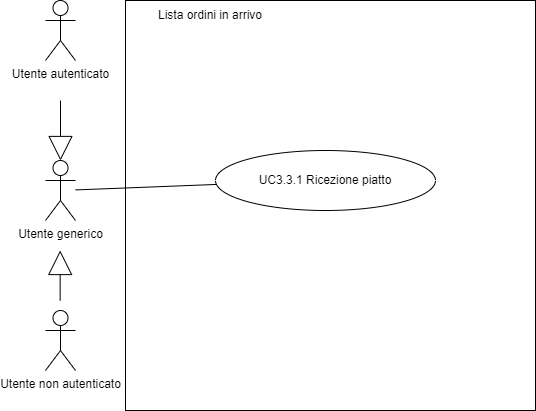
\includegraphics[scale=0.5]{usecase/tesi-uc333.drawio.png}
    \caption{Use Case - UC 3.3.1}
\end{figure}
\begin{itemize}
    \item \textbf{Descrizione:} L'utente marca un piatto in arrivo come ricevuto.
    \item \textbf{Attore Primario:} Untente generico.
    \item \textbf{Precondizione:} L'utente si trova dentro la sezione gestione ordini in arrivo e ha almeno un piatto nella lista in arrivo.
    \item \textbf{Postcondizione:} L'utente marca il piatto come arrivato diminuendo di 1 la sua quantità.
    \item \textbf{Scenrio principale:}
    \begin{itemize}
        \item L'utente si trova dentro la sezione gestione lista ordini in arrivo;
        \item L'utente clicca sul bottone "v" di un piatto;
        \item Viene diminuito di 1 la sua quantità.
    \end{itemize}
    \item \textbf{Scenrio alternativo:}
    \begin{itemize}
        \item L'utente si trova dentro la sezione gestione lista ordini in arrivo;
        \item L'utente clicca sul bottone "v" di un piatto con quantità uguale a 1;
        \item Viene diminuito di 1 la quantità del piatto e viene disabilitato il bottone.
    \end{itemize}
\end{itemize}

\section{Utente Non Autenticato}
\subsection{UC4 - Area personale}
\begin{figure}[H]
    \centering
    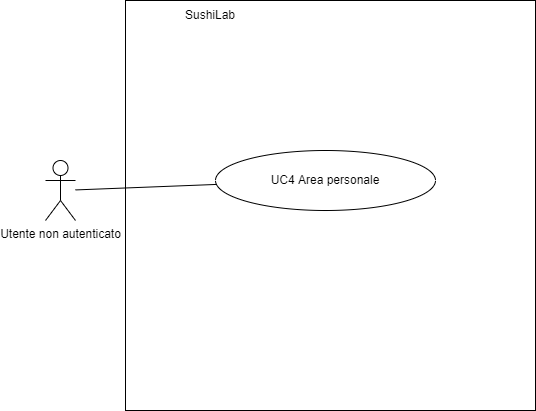
\includegraphics[scale=0.5]{usecase/tesi-uc4.drawio.png}
    \caption{Use Case - UC 4}
\end{figure}
\begin{itemize}
    \item \textbf{Descrizione:} L'utente visualizza la maschera dell'area personale.
    \item \textbf{Attore Primario:} Untente non autenticato.
    \item \textbf{Precondizione:} L'utente si trova dentro la web-app sushiLab.
    \item \textbf{Postcondizione:} Viene visualizzato la maschera dell'area personale.
    \item \textbf{Scenrio principale:}
    \begin{itemize}
        \item L'utente si trova dentro il sistema;
        \item Viene mostrato la mascheradell'area personale.
    \end{itemize}
\end{itemize}
\subsection{UC4.1 - Registrazione}
\begin{figure}[H]
    \centering
    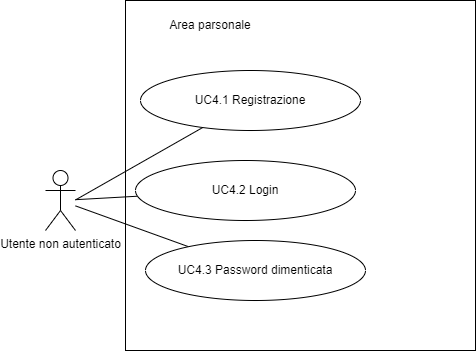
\includegraphics[scale=0.5]{usecase/tesi-uc41.drawio.png}
    \caption{Use Case - UC 4.1, UC 4.2, UC 4.3}
\end{figure}
\begin{itemize}
    \item \textbf{Descrizione:} L'utente viene registrato nella piattaforma.
    \item \textbf{Attore Primario:} Untente non autenticato.
    \item \textbf{Precondizione:} L'utente si trova dentro la web-app sushiLab.
    \item \textbf{Postcondizione:} Viene salvato i dati dell'utente inseriti durante la fase di registrazione nel data-base.
    \item \textbf{Scenrio principale:}
    \begin{itemize}
        \item L'utente si trova dentro l'area personale;
        \item L'utente clicca sul bottone registrati;
        \item Vine mostrato il form di registrazione;
        \item L'utente inserisce l'email;
        \item L'utente inserisce la password;
        \item L'utente ripete la password;
        \item L'utente clicca sul bottone registrati;
        \item Viene registrato correttamente l'account.
    \end{itemize}
    % \item \textbf{Estensioni:}
    % \begin{itemize}
    %     \item L'utente inserisce l'email già esistente nel data-base;
    %     \item Non viene registrato l'acocunt.
    % \end{itemize}
\end{itemize}
\subsection{UC4.2 - Login}
\begin{itemize}
    \item \textbf{Descrizione:} L'utente effettua login nella piattaforma.
    \item \textbf{Attore Primario:} Untente non autenticato.
    \item \textbf{Precondizione:} L'utente si trova dentro la web-app sushiLab.
    \item \textbf{Postcondizione:} Viene effettuato il login.
    \item \textbf{Scenrio principale:}
    \begin{itemize}
        \item L'utente si trova dentro l'area personale;
        \item L'utente inserisce l'email;
        \item L'utente inserisce la password;
        \item L'utente clicca sul bottone login;
        \item Viene effettuato il login correttamente.
    \end{itemize}
    % \item \textbf{Estensioni:}
    % \begin{itemize}
    %     \item L'utente inserisce l'email non esistente nel data-base o una password errata;
    %     \item Non viene effettuato il login.
    % \end{itemize}
\end{itemize}
\subsection{UC4.3 - Password dimenticata}
\begin{itemize}
    \item \textbf{Descrizione:} L'utente reimposta la password del proprio account.
    \item \textbf{Attore Primario:} Untente non autenticato.
    \item \textbf{Precondizione:} L'utente si trova dentro la web-app sushiLab.
    \item \textbf{Postcondizione:} Viene aggiornato la nuova password nel data-base.
    \item \textbf{Scenrio principale:}
    \begin{itemize}
        \item L'utente si trova dentro l'area personale;
        \item L'utente clicca sul bottone password dimenticata;
        \item Vine mostrato il form di recupero password;
        \item L'utente inserisce l'email;
        \item L'utente clicca sul bottone ottieni codice;
        \item L'utente arriva nel secondo form tramite il link mandato tramite email;
        \item L'utente inserisce la password;
        \item L'utente ripete la password;
        \item L'utente clicca sul bottone cambia password;
        \item Viene cambiato correttamente la password.
    \end{itemize}
    % \item \textbf{Estensioni:}
    % \begin{itemize}
    %     \item L'utente inserisce l'email non esistente nel data-base;
    %     \item Non viene effettuato il cambio password.
    % \end{itemize}
\end{itemize}
% \subsection{UCE1 - Email}
% \begin{itemize}
%     \item \textbf{Descrizione:} L'utente reimposta la password del proprio account.
%     \item \textbf{Attore Primario:} Untente non autenticato.
%     \item \textbf{Precondizione:} L'utente si trova dentro la web-app sushiLab.
%     \item \textbf{Postcondizione:} Viene aggiornato la nuova password nel data-base.
%     \item \textbf{Scenrio principale:}
%     \begin{itemize}
%         \item L'utente si trova dentro l'area personale;
%         \item L'utente clicca sul bottone password dimenticata;
%         \item Vine mostrato il form di recupero password;
%         \item L'utente inserisce l'email;
%         \item L'utente clicca sul bottone ottieni codice;
%         \item L'utente arriva nel secondo form tramite il link mandato tramite email;
%         \item L'utente inserisce la password;
%         \item L'utente ripete la password;
%         \item L'utente clicca sul bottone cambia password;
%         \item Viene cambiato correttamente la password.
%     \end{itemize}
% \end{itemize}
\section{Utente Autenticato}
\subsection{UC4.4 - Logout}
\begin{figure}[H]
    \centering
    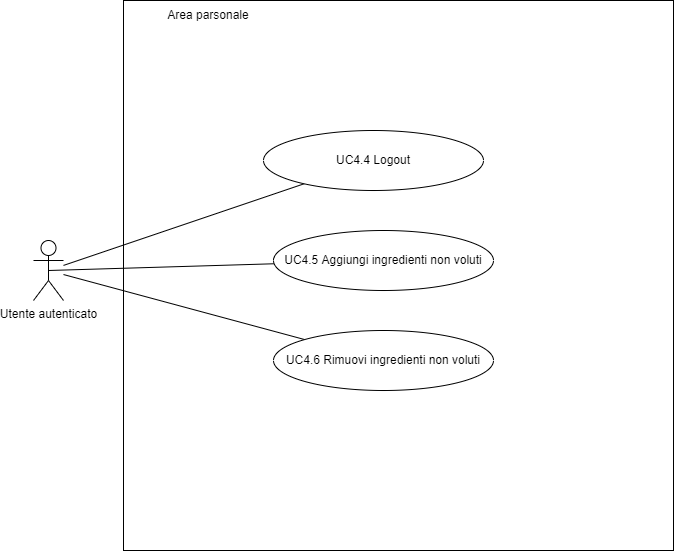
\includegraphics[scale=0.5]{usecase/tesi-uc42.drawio.png}
    \caption{Use Case - UC 4.4, UC4.5, UC4.6}
\end{figure}
\begin{itemize}
    \item \textbf{Descrizione:} L'utente effettua logout.
    \item \textbf{Attore Primario:} Untente autenticato.
    \item \textbf{Precondizione:} L'utente si trova dentro la web-app sushiLab ed ha effettuato la login.
    \item \textbf{Postcondizione:} Viene effettuato il logout.
    \item \textbf{Scenrio principale:}
    \begin{itemize}
        \item L'utente si trova dentro l'area personale;
        \item L'utente clicca sul bottone logout;
        \item Viene effettuato il logout dell'utente.
    \end{itemize}
\end{itemize}
\subsection{UC4.5 - Aggiungi ingredienti non voluti}
\begin{itemize}
    \item \textbf{Descrizione:} L'utente inserisce un ingrediente nella blacklist.
    \item \textbf{Attore Primario:} Untente autenticato.
    \item \textbf{Precondizione:} L'utente si trova dentro la web-app sushiLab  ha effettuato la login.
    \item \textbf{Postcondizione:} Viene inserito l'ingrediente nella blacklist.
    \item \textbf{Scenrio principale:}
    \begin{itemize}
        \item L'utente si trova dentro l'area personale;
        \item L'utente clicca sul bottone blacklist ingredienti;
        \item L'utente inserisce il nome del ingrediente;
        \item L'utente clicca sul bottone +;
        \item Viene inserito ingrediente nella blacklist.
    \end{itemize}
\end{itemize}
\subsection{UC4.6 - Rimuovi ingredienti non voluti}
\begin{itemize}
    \item \textbf{Descrizione:} L'utente rimuove un ingrediente dalla blacklist.
    \item \textbf{Attore Primario:} Untente autenticato.
    \item \textbf{Precondizione:} L'utente si trova dentro la web-app sushiLab  ha effettuato la login.
    \item \textbf{Postcondizione:} Viene rimosso l'ingrediente dalla blacklist.
    \item \textbf{Scenrio principale:}
    \begin{itemize}
        \item L'utente si trova dentro l'area personale;
        \item L'utente clicca sul bottone blacklist ingredienti;
        \item L'utente clicca sul bottone - di un ingrediente già esistente;
        \item Viene rimosso ingrediente dalla blacklist.
    \end{itemize}
\end{itemize}
\subsection{UC1.7 - Aggiungi preferiti}
\begin{figure}[H]
    \centering
    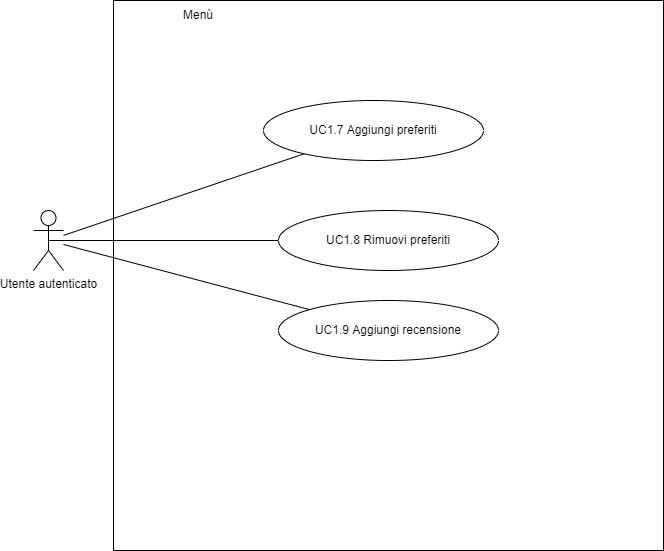
\includegraphics[scale=0.5]{usecase/tesi-uc111.drawio.png}
    \caption{Use Case - UC 1.7, UC1.8, UC1.9}
\end{figure}
\begin{itemize}
    \item \textbf{Descrizione:} L'utente aggiunge un piatto nella lista dei preferiti.
    \item \textbf{Attore Primario:} Untente autenticato.
    \item \textbf{Precondizione:} L'utente si trova dentro nella sezione menù.
    \item \textbf{Postcondizione:} Viene inserito il piatto nei preferiti.
    \item \textbf{Scenrio principale:}
    \begin{itemize}
        \item L'utente si trova nella sezione menù;
        \item L'utente clicca sul bottone "cuoricino grigio";
        \item Viene inserito il piatto nella lista dei preferiti.
    \end{itemize}
\end{itemize}
\subsection{UC1.8 - Rimuovi preferiti}
\begin{itemize}
    \item \textbf{Descrizione:} L'utente rimuove un piatto nella lista dei preferiti.
    \item \textbf{Attore Primario:} Untente autenticato.
    \item \textbf{Precondizione:} L'utente si trova dentro nella sezione menù.
    \item \textbf{Postcondizione:} Viene rimosso il piatto dalla lista dei preferiti.
    \item \textbf{Scenrio principale:}
    \begin{itemize}
        \item L'utente si trova nella sezione menù;
        \item L'utente clicca sul bottone "cuoricino rosa";
        \item Viene rimosso il piatto nella lista dei preferiti.
    \end{itemize}
\end{itemize}
\subsection{UC1.9 - Aggiungi recensione}
\begin{itemize}
    \item \textbf{Descrizione:} L'utente Aggiungi una recensione per un piatto.
    \item \textbf{Attore Primario:} Untente autenticato.
    \item \textbf{Precondizione:} L'utente si trova dentro nella sezione menù.
    \item \textbf{Postcondizione:} Viene inserito la recensione del piatto.
    \item \textbf{Scenrio principale:}
    \begin{itemize}
        \item L'utente si trova nella sezione menù;
        \item L'utente clicca su una delle 5 stelle;
        \item Viene inserito la recensione del piatto.
    \end{itemize}
\end{itemize}
% Durante la fase di analisi iniziale sono stati individuati alcuni possibili rischi a cui si potrà andare incontro.
% Si è quindi proceduto a elaborare delle possibili soluzioni per far fronte a tali rischi.\\

% \begin{risk}{Performance del simulatore hardware}
%     \riskdescription{le performance del simulatore hardware e la comunicazione con questo potrebbero risultare lenti o non abbastanza buoni da causare il fallimento dei test}
%     \risksolution{coinvolgimento del responsabile a capo del progetto relativo il simulatore hardware}
%     \label{risk:hardware-simulator} 
% \end{risk}

%**************************************************************
\section{Requisiti}
\subsection{Introduzione}
In base a quanto definito nell'analisi dei requisiti sono stati individuati una lista dei requisiti. Nella tabella si trovano tutti requisiti del progetto.
Il codice dei requisiti è così strutturato R(F/Q/V)(N/D/O) dove:
\begin{enumerate}
	\item[R =] requisito
    \item[F =] funzionale
    \item[Q =] qualitativo
    \item[V =] di vincolo
    \item[N =] obbligatorio (necessario)
    \item[D =] desiderabile
    \item[Z =] opzionale
\end{enumerate}
\subsection{Lista dei requisiti}
\begin{center}
    \rowcolors{2}{Cyan!10}{GreenYellow!10}
    \renewcommand{\arraystretch}{1.5}
    \begin{longtable}{ |p{1.5cm}|p{9cm}|p{1.5cm}|  }
        \hline
        \multicolumn{3}{|c|}{Tabella dei requisiti} \\
        \hline
        Codice&Requisito &Fonte \\
        \hline
        \endhead
        ROF1&L'utente può accedere al menù del ristorante&UC1 \\
        ROF2&All'utetne viene mostrato il menù del ristorante con tutte le categorie&UC1.1 \\
        ROF3&All'utetne viene mostrato il menù del ristorante con tutti piatti delle rispettive categorie di appartenenza&UC1.2 \\
        ROF4&L'utente può aumentare la quantità di un piatto nel menù&UC1.3 \\
        ROF5&L'utente può diminuire la quantità di un piatto nel menù&UC1.4 \\
        ROF&L'utente può impostare la visualizzazione dei piatti del menù nella modalità dettaglio&UC1.5 \\
        ROF&L'utente può impostare la visualizzazione dei piatti del menù nella modalità normale&UC1.6 \\
        ROF&L'utente può accedere alla maschera per la gestione tavolo &UC2 \\
        ROF&L'utente può generare la sessione del tavolo in cui si trova&UC2.1\\
        ROF&L'utente può unirsi alla sessione di un tavolo&UC2.2 \\
        ROF&L'utente può uscire dalla sessione di un tavolo&UC2.3\\
        ROF&L'utente può generare il QR-code della sessione del tavolo in cui si trova&UC2.4\\
        ROF&L'utente può accedere alla maschera per la gestione della lista ordini&UC3 \\
        ROF&All'utetne viene mostrato la lista ordini del tavolo&UC3.1 \\
        ROF&All'utetne viene mostrato la lista ordini personali &UC3.2 \\
        ROF&All'utetne viene mostrato la lista ordini in arrivo&UC3.3 \\
        ROF&L'utente può spostare la lista ordini del tavolo in arrivo &UC3.3.1 \\
        ROF&L'utente può generare il QR-code della lista ordini del tavolo in cui si trova &UC3.1.2 \\
        ROF&L'utente può impostare la visualizzazione dei piatti della lista ordini personali in modalità dettaglio&UC3.2.1 \\
        ROF&L'utente può marcare un piatto della lista ordini in arrivo come ricevuto&UC3.3.1 \\
        ROF&L'utente non autenticato può accedere all'area personale&UC4\\
        ROF&L'utente non autenticato deve riuscire ad inserire email, password e conferma password nel form di registrazione per effettuare la registrazione &UC4.1\\
        ROF&L'utente non autenticato deve riuscire ad inserire email e password nel form di login per effettuare la login &UC4.2\\
        ROF&L'utente non autenticato deve riuscire ad inserire la email e la nuova password nel form del password dimenticata&UC4.3\\
        ROF&L'utente autenticato deve riuscire ad effettuare la logout nell'area personale&UC4.4\\
        ROF&L'utente autenticato può aggiungere ingredienti non voluti nell'area personale&UC4.4\\
        ROF&L'utente autenticato può rimuovere ingredienti non voluti nell'area personale&UC4.4\\
        ROF&L'utente autenticato può aggiungere un piatto nella lista dei preferiti&UC4.4\\
        ROF&L'utente autenticato può rimuovere un piatto dalla lista dei preferiti&UC4.4\\
        ROF&L'utente autenticato può aggiungere una recensione per un piatto&UC1.7\\
        ROV&L'interfaccia utente del sistema dovrà essere sviluppato sfruttando il framework Angular&SyncLab\\
        ROV&Lo stile dell'interfaccia utente del sistema dovrà essere sviluppato sfruttando CSS-3&SyncLab\\
        ROV&Le chiamate API devono essere implementate tramite Stoplight&SyncLab\\
        ROV&È necessario dividire le varie maschere in componenti diversi di Angular&SyncLab\\
        ROV&La web-app dovrà funzionare sul browser Microsoft Edge dalla versione più recente&SyncLab\\
        ROV&La web-app dovrà funzionare sul browser Google Chrome dalla versione più recente&SyncLab\\
        ROV&La web-app dovrà funzionare sul browser Firefox dalla versione più recente&SyncLab\\
        ROV&La web-app dovrà funzionare sul browser Safari dalla versione più recente&SyncLab\\
        RDV&Il codice sorgente dovrà essere commentata&SyncLab\\
        ROQ&Il codice sorgente della piattaforma sarà reperibile su GitHub&SyncLab\\
        ROQ&Fornire una sezione tutorial che spieghi come si utilizza la web-app&SyncLab\\
       
\hline
\end{longtable}
\end{center}             % Kick-Off
% !TEX encoding = UTF-8
% !TEX TS-program = pdflatex
% !TEX root = ../tesi.tex

%**************************************************************
\chapter{Progettazione e codifica}
\label{cap:progettazione e codifica}
%**************************************************************

\intro{In questo capitolo vengono trattati la progettazione e codifica della parte front-end della web-app. Vengono elencati e descritti tutti i componenti della web-app e la loro funzionalità.}\\

\section{Progettazione}
\subsection{Architettura Angular}
Un'applicazione Angular è formata da un insieme di moduli, dove il modulo pricinpale è il modulo root, chiamato AppModule, che contiene più moduli di funzionalità. Un modulo di funzionalità è composto da un componente, che definisce la vista dell'utente.\\
Ogni componente possiede un template di HTML, dove viene definita il modello di vista, quando un utente effettua un click su un bottone, questo elemento HTML emette un evento di click al componente in cui si trova, questo componente esegue il metodo specifico al evento ricevuto, di seuito viene cambiato il metadata e modificato il codice HTML, una volta cambiata la struttura della pagina viene fatto il rendering della pagina e viene cambiata la vista dell'utente.\\
% Quindi un click su un bottone questo elemento HTML emette un evento di click al componente in cui si trova, questo componente esegue il metodo specifico al evento ricevuto, di seuito viene cambiato il metadata e viene aggiornato il template di HTML.\\
I componenti utilizzano dei servizi che forniscono funzionalità specifiche come il login di Auth.Service, ma non sono correlate direttamente alla vista, essi sono inseriti come delle dipendenze e grazie a questo rende il codice efficiente. Non solo i servizi sono riutilizzabili ma anche i componenti lo sono, dunque rende l'applicazione Angular più semplice da comprendere e manutenibile in futuro.\\
\begin{figure}[H]
    \centering
    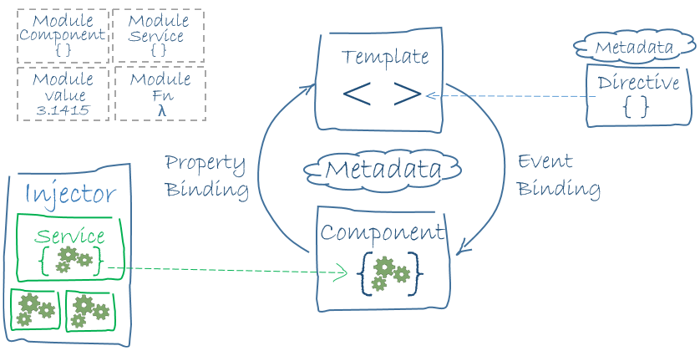
\includegraphics[scale=0.5]{angularArc.png}
    \caption{Architettura Angular}
\end{figure}
\subsection{Architettura SushiLab}
La web-app segue l'architettura spiegata precedentemente che è anche quello consigliato dal sito ufficiale di Angular.\\
La cartella principale della web-app è app che contiene tutti i componenti, i servizi e il root.\\ 
Per ogni componente si è creato una cartella per essa, in cui contiene il suoi file .ts per la logica, .html per la struttura, .scss per il layout di grafica e infine i suoi componenti figli. Per i componenti condivisi si è creato una cartella shared dove vengono salvati i componenti che sono utilizzati in più parti dell'applicazione.\\
Nella cartella \gls{restg} vengono salvati tutti i file service, in cui ci sono dei metodi che vengono chiamati in più componenti dell'applicazione al fine di massimizzare il riuso del codice.\\
Nella cartella assets vengono salvati le immagini e le icone utilizzate, in modo da fare utilizzare da tutti i componenti.\\
\begin{figure}[H]
    \centering
    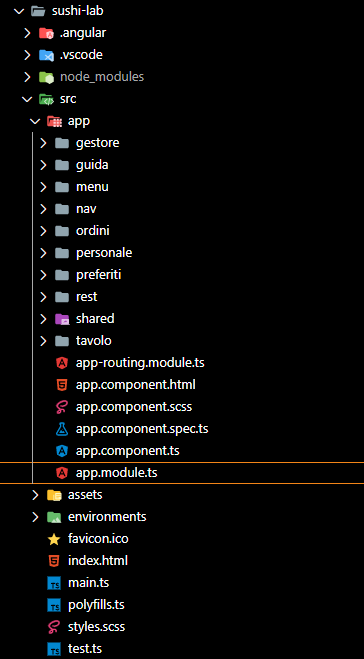
\includegraphics[scale=0.55]{struttura.png}
    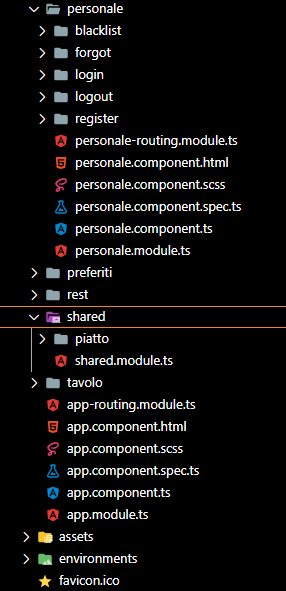
\includegraphics[scale=0.6]{struttura1.png}
    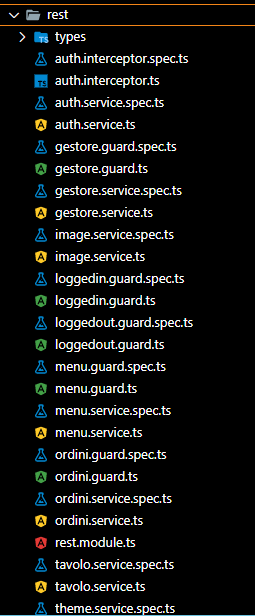
\includegraphics[scale=0.55]{struttura2.png}
    \caption{Struttura file SushiLab}
\end{figure}
\subsection{Progettazione delle viste}
All'inizio si è fatto un meeting con il tutor aziendale per chiarire le funzionalità e i requisiti che la web-app deve avere, dopo di che si è iniziato la progettazione dei mock-up delle viste tramite la editor di grafica online Figma.\\
Tramite il sistema di progettazione di Figma sono stati creati le bozze delle viste per chiarire i collegamenti tra di loro e i posizionamenti dei compoenti. 
Il posizionamento è scelto in base alla frequenza di click su di essa e si basa anche sulle viste dei web-app più popolari.
È stato deciso i seguenti aspetti:
\begin{itemize}
    \item I colori principali e lo sfondo della applicazione;
    \item Il bottone per la navbar è in alto a destra;
    \item Il logo della piattaforma in alto a sinistra;
    \item I bottoni, testi e form devono avere lo stesso stile e colore in base alla loro funzionalità;
    \item Lo stile del piatto in modalità dettaglio in menù e nella lista degli ordini personali è la stessa;
    \item Tutti le maschere hanno una visuale che utilizza la card.
\end{itemize}
\begin{figure}[H]
    \centering
    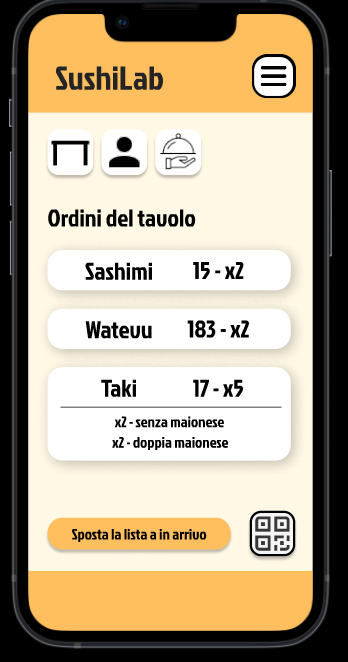
\includegraphics[scale=1]{figma.png}
    \caption{Figma SushiLab}
\end{figure}
\subsection{Progettazione API}
Durante il periodo di stage non era ancora presente il \gls{backendg} per l'applicativo, quindi si è deciso con l'azienda di progettare dei mock API per il testing utilizzando la piattaforma Stoplight.\\
La progettazione delle API sono molto semplici grazie all'interfaccia semplice di Stoplight, che permette di definire i path e i rispettivi metodi facilmente, e ai mock-up delle viste prima definite.\\
Per ogni chiamata \gls{restg} bisogna definire:
\begin{itemize}
    \item \textbf{Nome:} individua API;
    \item \textbf{Descrizione:} spiega in dettaglio la funzione della API;
    \item \textbf{Metodo:} definisce il tipo di chiamata, è stato usato:
    \begin{itemize}
        \item  \textbf{get:} per richiedere dei dati al server come la chiamata per ottenere il menù;
        \item  \textbf{post:} per inviare dei dati sintetici al server come i dati per login;
        \item  \textbf{delete:} per eliminare dei dati dal server come eliminazione della sessione di tavolo.
    \end{itemize}
    \item \textbf{Path:} definisce il percorso finale della API;
    \item \textbf{Risposta:} configura la risposta che ritorna la API, è stato usato:
    \begin{itemize}
        \item  \textbf{200:} richiesta andata a buon fine;
        \item  \textbf{201:} creazione andata a buon fine;
        \item  \textbf{204:} richiesta andata a buon fine ma il contenuto è vuoto;
        \item  \textbf{401:} non autorizzato;
        \item  \textbf{404:} non trovato;
        \item  \textbf{406:} non accettato;
        \item  \textbf{500:} errore interno.
    \end{itemize}
\end{itemize}
\begin{figure}[H]
    \centering
    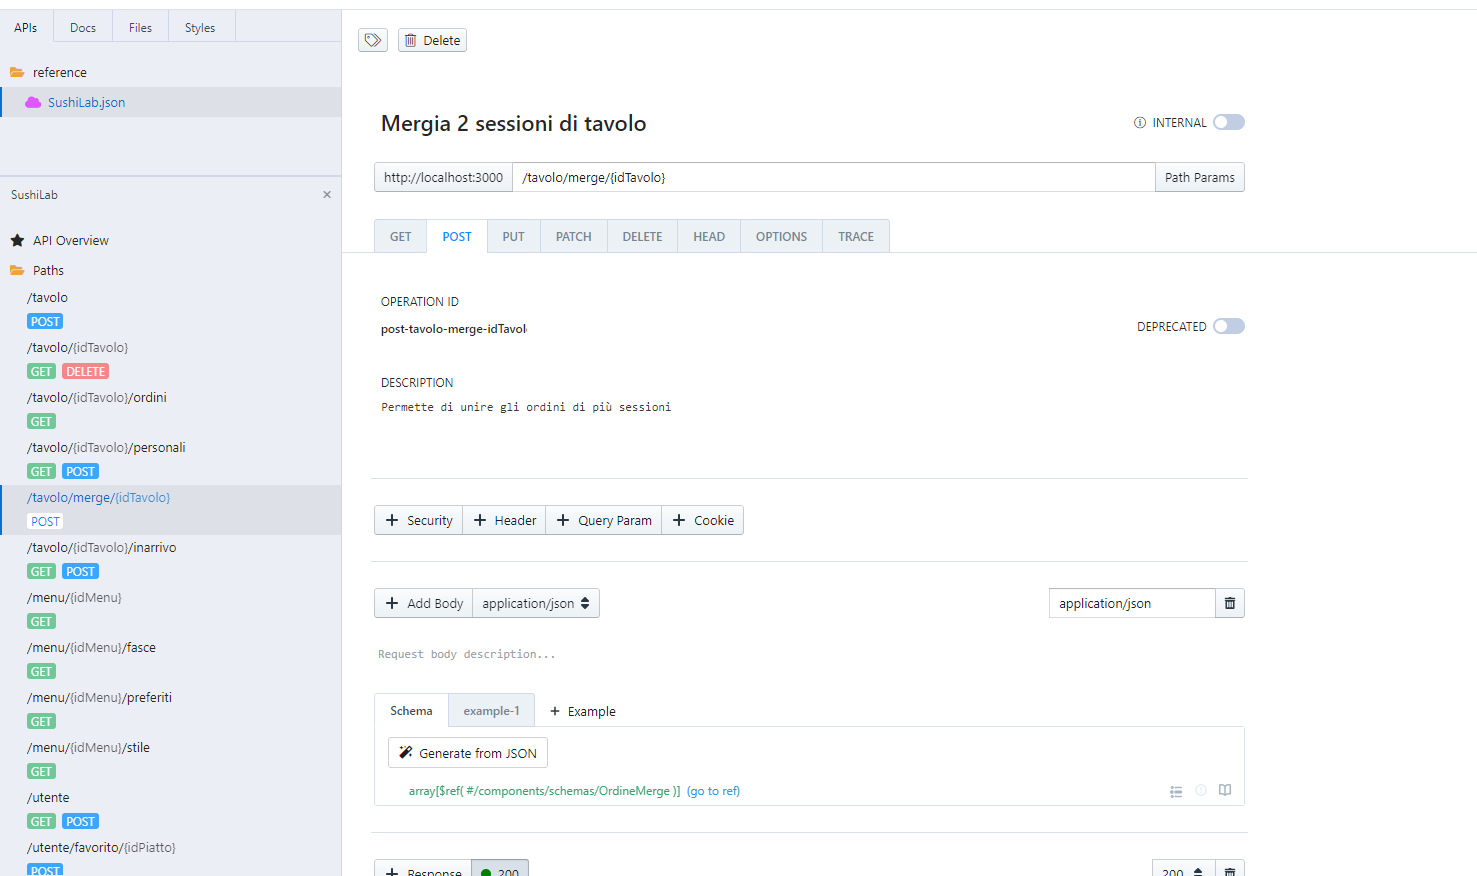
\includegraphics[scale=0.55]{stoplight.png}
    \caption{Stoplight SushiLab}
\end{figure}

\subsection{Progettazione dei componenti}
I componenti sono stati individuati tramite l'analisi dei requisiti e la progettazione delle viste. Ogni componente ha delle funzionalità specifiche e tutti assieme costruisce la web-app che copre tutti i requisiti richiesti.
\\
% {\hyperref[cap:menu.component]{Il secondo capitolo}}
\section{Codifica}
\subsection{Interfacce}
Dopo aver progettato i mock della visuale tramite figma e le API tramite stoplight ho iniziato la fase di codifica delle interfacce. La creazione dei template di default dei componenti è stato molto rapido grazie al command-line interface di Angular, utilizzando il comando 'ng generate component "nome del componente"' che crea una cartella contenente tutti i file necessari per il rendering del componente. Dopo la creazione dei file principali ho proceduto a modificare il component.ts, che rapprensenta la logica del componente, inserendo tutte le funzionalità che il componente deve avere. Una volta definito questo sono passato alla struttura e lo stile quindi a modificare il component.html e il component.css.
Tutte le interfacce, con le loro funzionalità e una descrizione dettagliata possono essere reperite nell'appendice {\hyperref[cap:appendice c]{C}}.
\subsubsection{Componenti service}
Per la comunicazione e gestione dei vari componenti vengono adoperati i file service. Per ogni servizio viene creato un file.service utilizzabile da uno o più component.\\
I servizi utilizzati sono:
\begin{itemize}
    \item auth.service: per gestire le autenticazioni;
    \item menu.service: per gestire tutte le funzionalità del menù;
    \item ordini.service: per gestire le ordinazioni;
    \item tavolo.service: per gestire le sessioni di tavolo;
    \item user.service: per gestire le funzionalità dell'area personale.
\end{itemize}
\subsubsection{Componenti guard}
Arrivato alla fine della codifica si definiscono i componenti guard, che permettono di imporre delle regole di accesso per la navigazione in un determinato componente. La verifica delle regole di guard avviene all'interno del metodo canActivate, appogiandosi ai diversi service e ai dati locali di sessione.             % Concept Preview
% !TEX encoding = UTF-8
% !TEX TS-program = pdflatex
% !TEX root = ../tesi.tex

%**************************************************************
\chapter{Verifica e validazione}
\label{cap:verifica}
%**************************************************************

\intro{In questa sezione vengono elencati i test di validazione effettuati e una descrizione della validazione.}\\

%**************************************************************
\section{Verifica}
Viene riportata una tabella dei test di unità sui vari componenti e sulle loro funzionalità, per ogni test viene assegnato un codice, il requisito associato, una descrizione e lo stato.
\begin{center}
    \rowcolors{2}{Cyan!10}{GreenYellow!10}
    \renewcommand{\arraystretch}{1.5}
    \begin{longtable}{ |p{1cm}|p{1.5cm}|p{9cm}|p{1.5cm}|  }
        \hline
        \hline
        Test&Requisito&Descrizione &Stato \\
        \hline
        \endhead
        T1&ROF1&Il componente menù viene creato&Passato \\
        T2&ROF3&Il componente piatto viene creato&Passato \\
        T3&ROF4&La quantità viene aumentata&Passato \\
        T4&ROF5&La quantità viene diminuita&Passato \\
        T5&ROF6&Il componente piatto viene visualizzato in modalità dettaglio&Passato \\
        % T1&ROF7&L'utente può impostare la visualizzazione dei piatti del menù nella modalità normale&Passato \\
        T6&ROF8&Il componente gestione del tavolo viene creato &Passato \\
        T7&ROF9&La sessione viene generata&Passato\\
        T8&ROF10&L'utente viene unito ad una sessione&Passato \\
        T9&ROF11&L'utente esce dalla sessione&Passato\\
        T10&ROF12&Il QR-code del tavolo viene generato&Passato\\
        T11&ROF13&Il componente gestione lista degli ordini viene creato&Passato\\
        % T1&ROF14&All'utente viene mostrato la lista degli ordini del tavolo&Passato\\
        % T1&ROF15&All'utente viene mostrato la lista degli ordini personali &Passato\\
        % T1&ROF16&All'utente viene mostrato la lista degli ordini in arrivo&Passato\\
        T12&ROF17&La lista degli ordini del tavolo viene spostato in arrivo&Passato\\
        T13&ROF18&Il QR-code della lista degli ordini viene generato &Passato\\
        % T1&ROF19&L'utente può impostare la visualizzazione dei piatti della lista degli ordini personali in modalità dettaglio&Passato\\
        T14&ROF20&Il piatto della lista degli ordini in arrivo viene marcato come arrivato&Passato\\
        T15&ROF21&Il componente area personale viene creato&Passato\\
        T16&ROF22&Il componente register viene creato&Passato\\
        T17&ROF22&I campi sbagliati del form di registrazione vengono evidenziati&Passato\\
        T18&ROF22&Il submit del form deve registrare l'utente&Passato\\
        T19&ROF23&Il componente login viene creato&Passato\\
        T20&ROF23&I campi sbagliati del form di login vengono evidenziati &Passato\\
        T21&ROF23&Il submit del form deve effettuare il login dell'utente &Passato\\
        T22&ROF24&Il componente forgot viene creato  &Passato\\
        T23&ROF24&I campi sbagliati del form di password dimenticata vengono evidenziati &Passato\\
        T24&ROF24&Il submit del form deve reimpostare la password&Passato\\
        T25&ROF25&Il componente logout viene creato&Passato\\
        T26&ROF25&Il click sul componente logout deve effettuare il logout dell'utente&Passato\\
        T27&ROF26&Il componente blacklist viene creato&Passato\\
        T28&ROF26&L'ingrediente viene inserito nella blacklist&Passato\\
        T29&ROF27&L'ingrediente viene rimosso dalla blacklist&Passato\\
        T30&ROF28&Il piatto viene aggiunto alla lista dei preferiti&Passato\\
        T31&ROF29&Il piatto viene rimosso dalla lista dei preferiti&Passato\\
        T32&ROF30&Il componente star viene creato&Passato\\
        T34&ROF30&La recensione viene generato correttamente&Passato\\
        T35&ROF31&Il componente lista preferiti viene creato&Passato\\
\hline
\caption{\label{tab:tabella dei test sui requisiti}Tabella dei test sui requisiti.}
\end{longtable}
\end{center}
\section{Validazione e collaudo}
Nell'ultima settimana dello stage ho controllato tutte le funzionalità implementate durante intero progetto, dove ho testato tutte le attività che sono svolgibili da un utente generale. Infine è stato mostrato il prodotto finale del progetto sushiLab al tutor aziendale con una demo completa di tutte le funzionalità della web-app.             % Product Prototype
% !TEX encoding = UTF-8
% !TEX TS-program = pdflatex
% !TEX root = ../tesi.tex

%**************************************************************
\chapter{Conclusioni}
\label{cap:conclusioni}
%**************************************************************
\section{Raggiungimento degli obiettivi}
\subsection{Obiettivi fissati}
Tutti gli obiettivi fissati all'inizio dello stage con il tutor aziendale sono stati raggiunti, oltre ai requisiti obbligatori sono stati soddisfatti anche i requisiti desiderabili e i facoltativi. Infatti la web-app fonisce tutte le funzionalità richieste e offre inoltre la possibilità di salvare i piatti nella lista dei preferiti, filtrare il menù rimuovendo i piatti contenenti gli ingredienti presenti nella blacklist e fornire una recensione ad un piatto.
\begin{center}
    \rowcolors{2}{Cyan!10}{GreenYellow!10}
    \renewcommand{\arraystretch}{1.5}
    \begin{longtable}{ |p{1.5cm}|p{9cm}|p{2cm}|  }
        \hline
        \multicolumn{3}{|c|}{Obiettivi fissati} \\
        \hline
        Codice&Descrizione &Esito \\
        \hline
        \endhead
        O01&Acquisizione competenze sulle tematiche sopra descritte&Superato \\
        O02&Capacità di raggiungere gli obiettivi richiesti in autonomia seguendo il cronoprogramma&Superato\\
        O03&Portare a termine le implementazioni previste con una percentuale di superamento pari al 80\%&Superato\\
        D01&Portare a termine le implementazioni previste con una percentuale di superamento pari al 100\%&Superato\\
        F01&Apportare un valore aggiunto al gruppo di lavoro durante le fasi di progettazione delle interfacce&Superato\\
\hline
\caption{\label{tab:tabella raggiungimento obiettivi fissati}Tabella del raggiungimento degli obiettivi fissati.}
\end{longtable}
\end{center}
\pagebreak

\subsection{Svolgimento del lavoro}
I lavori pianificati per le prime settimane di stage sono stati svolti senza particolari difficoltà, infatti le attività di studio e formazione sono terminate con un piccolo anticipo rispetto alla pianificazione e il tempo risparmiato è stato utilizzato alla fine per implementare le funzionalità aggiuntive. Questo guadagno di tempo è dovuto ad una buona familiarità con i linguaggi di programmazione acquisita durante gli anni di studio nell'ambito dell'informatica.\\
La fase di progettazione ed implementazione delle maschere è risultata più rapida del previsto anche grazie alla mia esperienza pregressa come cameriere in un ristorante sushi.\\
La parte che ha impiegato più ore di quelle previste è stata la fase di integrazione tra le varie maschere dove bisognava mantenere i dati salvati di ogni pagina, questo problema è stato risolto grazie ai componenti service forniti da Angular e al local storage del browser. Un altro strumento che ha dato un grande aiuto è stato discord perché ci ha permesso di comunicare facilmente con altri collaboratori del progetto.\\
\begin{center}
    \rowcolors{2}{Cyan!10}{GreenYellow!10}
    \renewcommand{\arraystretch}{1.5}
    \begin{longtable}{ |p{3cm}|p{9cm}|  }
        \hline
        Settimana&Attività \\
        \hline
        \endhead
        Prima settimana&\begin{itemize}
            \item Incontro con il tutor aziendale e i collaboratori
            \item Identificazione dei requisiti
            \item Formazione su strumenti di lavoro
            \item Ripasso HTML5, JavaScript e css
        \end{itemize}\\
        Seconda settimana& \begin{itemize}
            \item Formazione su Spring Core
            \item Formazione su Spring Boot
            \item Formazione su linguaggio TypeScript
            \item Formazione su Angular components
        \end{itemize}\\ 
        Terza settimana&\begin{itemize}
            \item Formazione su Angular data biding e pipes
            \item Formazione su Angular routing e forms
            \item Formazione su Angular lifecycle hooks
            \item Analisi dei requisiti
        \end{itemize}\\
        Quarta settimana&\begin{itemize}
            \item Progettazione delle interfacce tramite Figma
            \item Indentificazione dei colori della web-app
            \item Formazione sulla libreria Angular material
            \item Progettazione maschera d'accesso
        \end{itemize}\\
        Quinta settimana&\begin{itemize}
            \item Progettazione navbar
            \item Progettazione maschera menù
            \item Progettazione maschera gestione del tavolo
            \item Progettazione maschera gestione degli ordini
            \item Progettazione API
        \end{itemize}\\
        Sesta settimana&\begin{itemize}
            \item Progettazione componenti service
            \item Realizzazione funzionamento merge ordini
            \item Realizzazione funzionamento sposta ordini
            \item Progettazione componenti guard
        \end{itemize}\\
        Settima settimana&\begin{itemize}
            \item Integrazione dei componenti
            \item Decorazione finale della web-app
        \end{itemize}\\
        Ottava settimana&\begin{itemize}
            \item Verifica e validazione della web-app
            \item Documentazione analisi tecnica
            \item Collaudo finale
        \end{itemize}\\
\hline
\caption{\label{tab:tabella consuntivo lavoro}Tabella del consuntivo di lavoro.}
\end{longtable}
\end{center}
\pagebreak
%**************************************************************
% \section{Consuntivo finale}

%**************************************************************
% \section{Raggiungimento degli obiettivi}

%**************************************************************
\section{Conoscenze acquisite}
Durante lo stage nell'azienda SyncLab, ho acquisito nuove conoscenze tecniche.\\
Ho imparato ad usare Angular che è uno dei più famosi framework per lo sviluppo front-end nelle applicazioni. L'apprendimento di Angular è stato svolto principalmente in autonomia, consultando vari siti web e video a tema, ottenendo così una maggiore comprensione del framework.\\
Durante la fase di testing ho approfondito il framework Spring di Java al fine di progettare dei mock delle \gls{apig} che rispecchiano il più possibile l'implementazione del back-end futuro.\\
Lavorare in Angular mi ha dato la possibilità di imparare TypeScript, ciò mi ha permesso di avere una visione più ampia dei problemi che riguardano JavaScript, come il sistema dei tipi e il processo di debugging.\\
Ogni settimana è stato fatto un incontro in sede con il tutor aziendale, dove si è discusso l'avanzamento della web-app, le difficoltà e la ripianificazione della settimana seguente in caso di cambiamenti, ciò mi ha permesso di familiarizzare con il metodo Agile.\\
% Tutto questo ha consolidato le mie competenze di programmazione comprese durante gli anni di studio e mi ha dato tanti notevoli insegnamenti.
%**************************************************************

% fare come Stafa
\section{Valutazione}
\subsection{L'azienda}
Durante il processo di sviluppo tutte le persone dell'azienda sono state molto disponibili, inizialmente mi hanno illustrato il back-end di un grande progetto fornendomi consigli su come scrivere codice al fine di facilitare il debugging. Il tutor aziendale è sempre stato molto gentile e mi ha dato la possibilità di lavolare sul front-end, che è sempre stato il mio ambito di sviluppo preferito.\\
Infine tutto ciò mi ha permesso di imparare a lavorare con scadenze rigorose come accade dentro ad un team vero e proprio.\\
\subsection{Personale}
Lo stage mi ha ampliamente soddisfatto, mi ha fatto conoscere meglio l'ambiente di lavoro di un programmatore permettendomi di usare tutte le competenze acquisite durante il corso di studio universitario.\\
Durante il tirocinio ho visto l'intero processo di sviluppo di un applicativo, partendo da un problema reale arrivando all'implementazione della web-app, questo mi è stato particolarmente importante per il mio avanzamento professionale da programmatore.
Arrivando alla fine, l'intera esperienza dello stage è più che positiva, ritengo che il tirocinio sia molto importante per uno studente, poiché permette di sfruttare e valutare le proprie conoscenze acquisite e in particolare per capire e riflettere sul percorso di studio scelto, infatti lo stage mi ha confermato di voler continuare la carriera lavorativa nell'ambito dello sviluppo.             % Product Design Freeze e SOP
\input{capitoli/capitolo-7}             % Conclusioni
\appendix                               
% !TEX encoding = UTF-8
% !TEX TS-program = pdflatex
% !TEX root = ../tesi.tex

%**************************************************************
\chapter{Descrizione dettagliata dei casi d'uso}
\label{cap:appendice a}
%**************************************************************
In questa sezione verranno descritti tutti i casi d'uso dettagliamente.
La descrizione generale dei casi d'uso è reperibile alla sezione 3.2.\\

% \epigraph{Citazione}{Autore della citazione}
\textbf{Utente generico}\\
\textbf{UC1 - Visualizza menù}
% \begin{figure}[H]
%     \centering
%     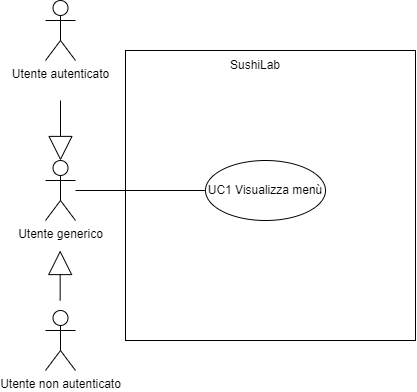
\includegraphics[scale=0.5]{usecase/tesi-uc1.drawio.png}
%     \caption{Use Case - UC 1}
% \end{figure}
\begin{itemize}
    \item \textbf{Descrizione:} L'utente visualizza il menù del ristorante.
    \item \textbf{Attore Primario:}L'utente generico.
    \item \textbf{Precondizione:} L'utente si trova dentro la web-app.
    \item \textbf{Postcondizione:} Viene visualizzato il menù del ristorante.
    \item \textbf{Scenario principale:}
    \begin{itemize}
        \item L'utente si trova dentro il sistema;
        \item L'utente clicca sul bottone menù;
        \item Viene mostrato il menù del ristorante.
    \end{itemize}
\end{itemize}
\textbf{UC1.1 - Visualizza categorie}
% \begin{figure}[H]
%     \centering
%     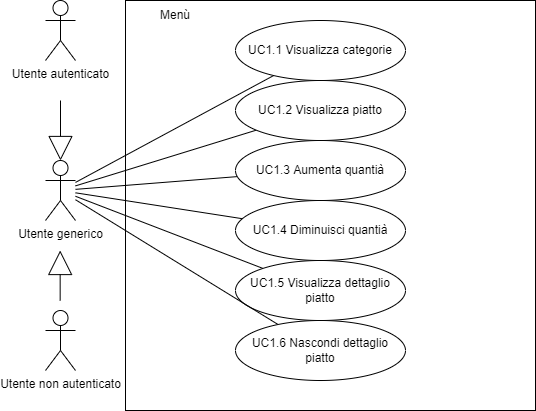
\includegraphics[scale=0.5]{usecase/tesi-uc11.drawio.png}
%     \caption{Use Case - UC 1.1, UC 1.2, UC 1.3, UC 1.4, UC 1.5, UC 1.6}
% \end{figure}
\begin{itemize}
    \item \textbf{Descrizione:} L'utente visualizza le categorie del menù.
    \item \textbf{Attore Primario:}L'utente generico.
    \item \textbf{Precondizione:} L'utente si trova dentro la sezione menù.
    \item \textbf{Postcondizione:} Vengono visualizzati i nomi delle categorie.
    \item \textbf{Scenario principale:}
    \begin{itemize}
        \item L'utente si trova nella sezione menù;
        \item Vengono mostrate le categorie del menù.
    \end{itemize}
\end{itemize}
\textbf{UC1.2 - Visualizza piatto}
\begin{itemize}
    \item \textbf{Descrizione:} L'utente visualizza i piatti del menù mostrando il numero, nome, prezzo, ingredienti, allergeni, limitazioni e la quantità. La quantità di default è 0 ed indica che il piatto non è ancora stato ordinato.
    \item \textbf{Attore Primario:} L'utente generico.
    \item \textbf{Precondizione:} L'utente si trova dentro la sezione menù.
    \item \textbf{Postcondizione:} Vengono visualizzati i piatti del menù.
    \item \textbf{Scenario principale:}  
    \begin{itemize}
        \item L'utente si trova nella sezione menù;
        \item Vengono mostrati i piatti del menù.
    \end{itemize}
\end{itemize}
\textbf{UC1.3 - Aumenta quantità}
\begin{itemize}
    \item \textbf{Descrizione:} L'utente aumenta la quantità di un piatto.
    \item \textbf{Attore Primario:}L'utente generico.
    \item \textbf{Precondizione:} L'utente si trova nella sezione menù o lista degli ordini personali.
    \item \textbf{Postcondizione:} Viene aggiunto il piatto specifico con la quantità aggiornata negli ordini.
    \item \textbf{Scenario principale:}
    \begin{itemize}
        \item L'utente si trova nella sezione menù;
        \item L'utente clicca sul bottone + di un piatto;
        \item Viene aggiunto il piatto negli ordini.
    \end{itemize}
    \item \textbf{Scenario alternativo:}
    \begin{itemize}
        \item L'utente si trova nella sezione menù o nella lista degli ordini personali;
        \item L'utente clicca sul bottone + di un piatto che è già presente negli ordini;
        \item Viene aumentata la quantità del piatto negli ordini.
    \end{itemize}
\end{itemize}
\textbf{UC1.4 - Diminuisci quantità}
\begin{itemize}
    \item \textbf{Descrizione:} L'utente dimiuisce la quantità di un piatto.
    \item \textbf{Attore Primario:}L'utente generico.
    \item \textbf{Precondizione:} L'utente si trova dentro la sezione menù o nella lista degli ordini personali.
    \item \textbf{Postcondizione:} Viene dimiuita la quantità del piatto specifico negli ordini.
    \item \textbf{Scenario principale:}
    \begin{itemize}
        \item L'utente si trova nella sezione menù o nella lista degli ordini personali;
        \item L'utente clicca sul bottone - di un piatto con quantità maggiore di 1;
        \item Viene diminuita la quantità del piatto negli ordini.
    \end{itemize}
    \item \textbf{Scenario alternativo:}
    \begin{itemize}
        \item L'utente si trova nella sezione menù o nella lista degli ordini personali;
        \item L'utente clicca sul bottone - di un piatto con quantità uguale a 1;
        \item Viene rimosso il piatto dagli ordini.
    \end{itemize}
\end{itemize}
\textbf{UC1.5 - Visualizza dettaglio piatto}
\begin{itemize}
    \item \textbf{Descrizione:} L'utente visualizza i dettagli di un piatto nel menù, mostrando la recensione del piatto e il text-box per inserire una nota.
    \item \textbf{Attore Primario:}L'utente generico.
    \item \textbf{Precondizione:} L'utente si trova dentro la sezione menù.
    \item \textbf{Postcondizione:} Vengono visualizzati i dettagli di un piatto specifico.
    \item \textbf{Scenario principale:}  
    \begin{itemize}
        \item L'utente si trova nella sezione menù;
        \item L'utente clicca sul bottom mostra dettagli;
        \item Vengono mostrati i dettagli di un piatto.
    \end{itemize}
\end{itemize}
\textbf{UC1.6 - Nascondi dettaglio piatto}
\begin{itemize}
    \item \textbf{Descrizione:} L'utente nasconde i dettagli di un piatto specifico.
    \item \textbf{Attore Primario:}L'utente generico.
    \item \textbf{Precondizione:} L'utente si trova dentro la sezione menù con un piatto in modalità dettaglio.
    \item \textbf{Postcondizione:} Vengono nascosti i dettagli del piatto specifico.
    \item \textbf{Scenario principale:}  
    \begin{itemize}
        \item L'utente si trova nella sezione menù;
        \item L'utente clicca sul bottom nascondi dettagli;
        \item Vengono nascosti i dettagli del piatto.
    \end{itemize}
\end{itemize}
\textbf{UC2 - gestione del tavolo}
% \begin{figure}[H]
%     \centering
%     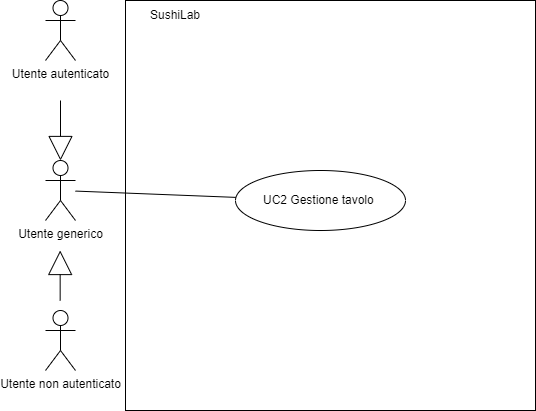
\includegraphics[scale=0.5]{usecase/tesi-uc2.drawio.png}
%     \caption{Use Case - UC 2}
% \end{figure}
\begin{itemize}
    \item \textbf{Descrizione:} L'utente visualizza la maschera di gestione del tavolo.
    \item \textbf{Attore Primario:}L'utente generico.
    \item \textbf{Precondizione:} L'utente si trova dentro la web-app.
    \item \textbf{Postcondizione:} Viene visualizzata la maschera di gestione del tavolo.
    \item \textbf{Scenario principale:}
    \begin{itemize}
        \item L'utente si trova dentro il sistema;
        \item L'utente clicca sul bottone gestione del tavolo nella navbar;
        \item Viene mostrata la maschera di gestione del tavolo.
    \end{itemize}
\end{itemize}
\textbf{UC2.1 - Generazione sessione tavolo}
% \begin{figure}[H]
%     \centering
%     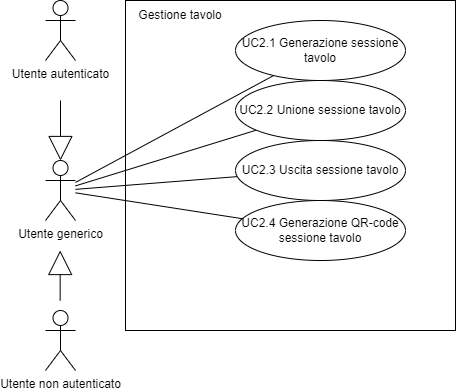
\includegraphics[scale=0.5]{usecase/tesi-uc21.drawio.png}
%     \caption{Use Case - UC 2.1, UC 2.2, UC 2.3, UC 2.4}
% \end{figure}
\begin{itemize}
    \item \textbf{Descrizione:} L'utente genera la sessione del tavolo.
    \item \textbf{Attore Primario:}L'utente generico.
    \item \textbf{Precondizione:} L'utente si trova dentro la sezione gestione del tavolo.
    \item \textbf{Postcondizione:} L'utente entra nella sessione generata del tavolo.
    \item \textbf{Scenario principale:}
    \begin{itemize}
        \item L'utente si trova dentro la sezione gestione del tavolo;
        \item L'utente clicca sul bottone crea sessione;
        \item Viene creata la sessione;
        \item L'utente viene inserito nella sessione creata.
    \end{itemize}
\end{itemize}
\textbf{UC2.2 - Unione sessione tavolo}
\begin{itemize}
    \item \textbf{Descrizione:} L'utente si unisce alla sessione del tavolo.
    \item \textbf{Attore Primario:}L'utente generico.
    \item \textbf{Precondizione:} L'utente si trova dentro la sezione gestione del tavolo.
    \item \textbf{Postcondizione:} L'utente entra nella sessione che è stata inserita.
    \item \textbf{Scenario principale:}
    \begin{itemize}
        \item L'utente si trova dentro la sezione gestione del tavolo;
        \item L'utente clicca sul bottone unisciti a una sessione;
        \item L'utente inserisce il numero della sessione;
        \item L'utente clicca sul bottone unisciti;
        \item L'utente viene inserito nella sessione.
    \end{itemize}
    % \item \textbf{Scenario alternativo:}
    % \begin{itemize}
    %     \item L'utente si trova dentro la sezione gestione del tavolo;
    %     \item L'utente clicca sul bottone unisciti a una sessione;
    %     \item L'utente inserisce il numero della sessione inesistente;
    %     \item L'utente clicca sul bottone unisciti;
    %     \item L'utente non viene inserito nella sessione.
    % \end{itemize}
\end{itemize}
\textbf{UC2.3 - Uscita sessione tavolo}
\begin{itemize}
    \item \textbf{Descrizione:} L'utente esce dalla sessione del tavolo.
    \item \textbf{Attore Primario:}L'utente generico.
    \item \textbf{Precondizione:} L'utente si trova dentro la sezione gestione del tavolo ed è dentro ad una sessione.
    \item \textbf{Postcondizione:} L'utente esce dalla sessione del tavolo.
    \item \textbf{Scenario principale:}
    \begin{itemize}
        \item L'utente si trova dentro la sezione gestione del tavolo;
        \item L'utente clicca sul bottone esci dalla sessione;
        \item L'utente viene rimosso dalla sessione.
    \end{itemize}
\end{itemize}
\textbf{UC2.4 - Generazione QR-code sessione tavolo}
\begin{itemize}
    \item \textbf{Descrizione:} L'utente genera il QR-code dalla sessione del tavolo per mostrarlo agli altri al fine di farli unire scansionando il codice-QR.
    \item \textbf{Attore Primario:}L'utente generico.
    \item \textbf{Precondizione:} L'utente si trova dentro la sezione gestione del tavolo ed è dentro ad una sessione.
    \item \textbf{Postcondizione:} L'utente genera il QR-code dalla sessione del tavolo.
    \item \textbf{Scenario principale:}
    \begin{itemize}
        \item L'utente si trova dentro la sezione gestione del tavolo;
        \item L'utente genera il QR-code della sessione;
        \item Viene mostrato il QR-code;
    \end{itemize}
\end{itemize}
\textbf{UC3 - lista degli ordini}
% \begin{figure}[H]
%     \centering
%     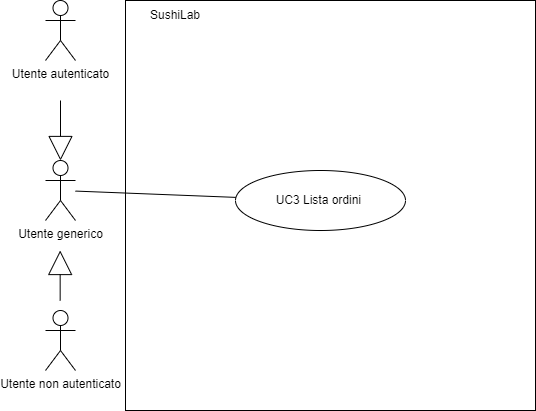
\includegraphics[scale=0.5]{usecase/tesi-uc3.drawio.png}
%     \caption{Use Case - UC 3}
% \end{figure}
\begin{itemize}
    \item \textbf{Descrizione:} L'utente visualizza la maschera di gestione degli ordini.
    \item \textbf{Attore Primario:}L'utente generico.
    \item \textbf{Precondizione:} L'utente si trova dentro ad una sessione del tavolo.
    \item \textbf{Postcondizione:} Viene visualizzata la maschera di gestione degli ordini.
    \item \textbf{Scenario principale:}
    \begin{itemize}
        \item L'utente si trova dentro il sistema con una sessione del tavolo attiva;
        \item L'utente clicca sul bottone lista degli ordini nella navbar;
        \item Viene mostrata la maschera di gestione degli ordini.
    \end{itemize}
\end{itemize}
\textbf{UC3.1 - Visualizza lista degli ordini del tavolo}
% \begin{figure}[H]
%     \centering
%     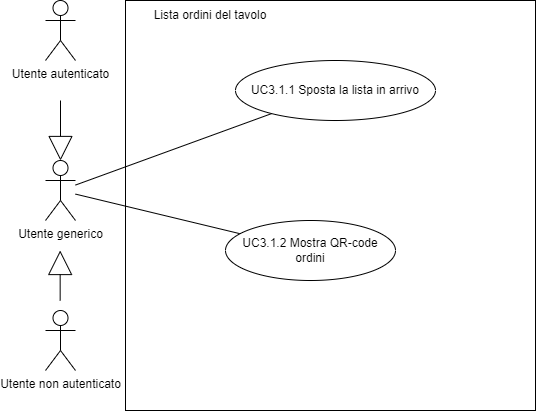
\includegraphics[scale=0.5]{usecase/tesi-uc311.drawio.png}
%     \caption{Use Case - UC 3.1, UC 3.2, UC 3.3}
% \end{figure}
\begin{itemize}
    \item \textbf{Descrizione:} L'utente visualizza la lista degli ordini della sessione del tavolo in cui si trova. 
    \item \textbf{Attore Primario:}L'utente generico.
    \item \textbf{Precondizione:} L'utente si trova dentro la sezione lista degli ordini.
    \item \textbf{Postcondizione:} Viene visualizzata la lista degli ordini del tavolo.
    \item \textbf{Scenario principale:}
    \begin{itemize}
        \item L'utente si trova dentro la sezione gestione degli ordini;
        \item L'utente clicca sul bottone "tavolo";
        \item Viene mostrata la lista dei piatti ordinati del tavolo.
    \end{itemize}
\end{itemize}
\textbf{UC3.2 - Visualizza lista degli ordini personali}
\begin{itemize}
    \item \textbf{Descrizione:} L'utente visualizza la lista degli ordini personali.
    \item \textbf{Attore Primario:}L'utente generico.
    \item \textbf{Precondizione:} L'utente si trova dentro la sezione lista degli ordini.
    \item \textbf{Postcondizione:} Viene visualizzata la lista degli ordini personali.
    \item \textbf{Scenario principale:}
    \begin{itemize}
        \item L'utente si trova dentro la sezione gestione degli ordini;
        \item L'utente clicca sul bottone "personali";
        \item Viene mostrata la lista dei piatti ordinati dall'utente stesso.
    \end{itemize}
\end{itemize}
\textbf{UC3.3 - Visualizza lista degli ordini in arrivo}
\begin{itemize}
    \item \textbf{Descrizione:} L'utente visualizza la lista degli ordini in arrivo.
    \item \textbf{Attore Primario:}L'utente generico.
    \item \textbf{Precondizione:} L'utente si trova dentro la sezione lista degli ordini.
    \item \textbf{Postcondizione:} Viene visualizzata la lista degli ordini in arrivo.
    \item \textbf{Scenario principale:}
    \begin{itemize}
        \item L'utente si trova dentro la sezione gestione degli ordini;
        \item L'utente clicca sul bottone "in arrivo";
        \item Viene mostrata la lista dei piatti in arrivo.
    \end{itemize}
\end{itemize}
\textbf{UC3.1.1 - Sposta la lista in arrivo}
\begin{itemize}
    \item \textbf{Descrizione:} L'utente sposta la lista degli ordini in arrivo.
    \item \textbf{Attore Primario:}L'utente generico.
    \item \textbf{Precondizione:} L'utente si trova dentro la sezione lista degli ordini del tavolo.
    \item \textbf{Postcondizione:} Viene spostata la lista degli ordini del tavolo in arrivo.
    \item \textbf{Scenario principale:}
    \begin{itemize}
        \item L'utente si trova dentro la sezione gestione degli ordini del tavolo;
        \item L'utente clicca sul bottone sposta la lista in arrivo;
        \item Viene spostata la lista dei piatti ordinati personali in modalità dettaglio;
        \item Viene mostrato all'utente il messaggio "ordini spostati correttamente".
    \end{itemize}
\end{itemize}
\textbf{UC3.1.2 - Mostra QR-code ordini}
\begin{itemize}
    \item \textbf{Descrizione:} L'utente genera il QR-code della lista degli ordini per dopo mostrarlo al cameriere.
    \item \textbf{Attore Primario:}L'utente generico.
    \item \textbf{Precondizione:} L'utente si trova dentro la sezione lista degli ordini del tavolo.
    \item \textbf{Postcondizione:} Viene mostrato il QR-code della lista degli ordini.
    \item \textbf{Scenario principale:}
    \begin{itemize}
        \item L'utente si trova dentro la sezione gestione degli ordini del tavolo;
        \item L'utente clicca sul bottone QR-code;
        \item Viene generato il QR-code degli ordini;
        \item Viene mostrato il QR-code.
    \end{itemize}
\end{itemize}
\textbf{UC3.2.1 - Visualizza in dettaglio lista degli ordini personali}
\begin{figure}[H]
    \centering
    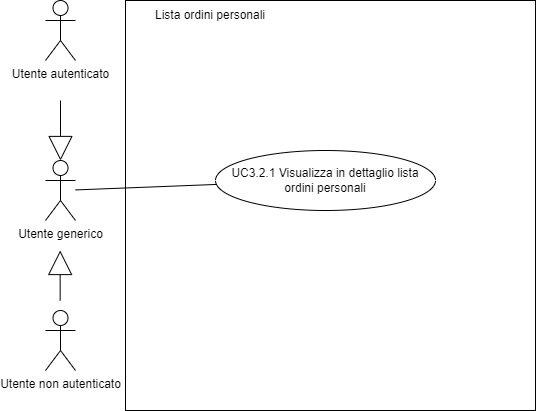
\includegraphics[scale=0.5]{usecase/tesi-uc322.drawio.png}
    \caption{Use Case - UC 3.2.1}
\end{figure}
\begin{itemize}
    \item \textbf{Descrizione:} L'utente visualizza la lista degli ordini personali in modalità dettaglio.
    \item \textbf{Attore Primario:}L'utente generico.
    \item \textbf{Precondizione:} L'utente si trova dentro la sezione lista degli ordini personali.
    \item \textbf{Postcondizione:} Viene visualizzata la lista degli ordini personali con i piatti in modalità dettaglio.
    \item \textbf{Scenario principale:}
    \begin{itemize}
        \item L'utente si trova dentro la sezione gestione degli ordini personali;
        \item L'utente clicca sul bottone "lente" con il +;
        \item Viene mostrata la lista dei piatti ordinati personali in modalità dettaglio.
    \end{itemize}
\end{itemize}
\textbf{UC3.3.1 - Ricezione piatto}
% \begin{figure}[H]
%     \centering
%     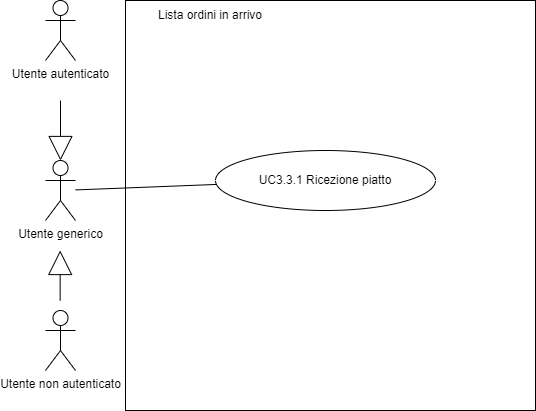
\includegraphics[scale=0.5]{usecase/tesi-uc333.drawio.png}
%     \caption{Use Case - UC 3.3.1}
% \end{figure}
\begin{itemize}
    \item \textbf{Descrizione:} L'utente marca un piatto in arrivo come ricevuto.
    \item \textbf{Attore Primario:}L'utente generico.
    \item \textbf{Precondizione:} L'utente si trova dentro la sezione gestione degli ordini in arrivo e ha almeno un piatto nella lista in arrivo.
    \item \textbf{Postcondizione:} L'utente marca il piatto come arrivato diminuendo di 1 la sua quantità.
    \item \textbf{Scenario principale:}
    \begin{itemize}
        \item L'utente si trova dentro la sezione gestione lista degli ordini in arrivo;
        \item L'utente clicca sul bottone "v" di un piatto;
        \item Viene diminuita di 1 la sua quantità.
    \end{itemize}
    \item \textbf{Scenario alternativo:}
    \begin{itemize}
        \item L'utente si trova dentro la sezione gestione lista degli ordini in arrivo;
        \item L'utente clicca sul bottone "v" di un piatto con quantità uguale a 1;
        \item Viene diminuita di 1 la quantità del piatto e viene disabilitato il bottone.
    \end{itemize}
\end{itemize}

\textbf{Utente non autenticato}\\
\textbf{UC4 - Area personale}
\begin{figure}[H]
    \centering
    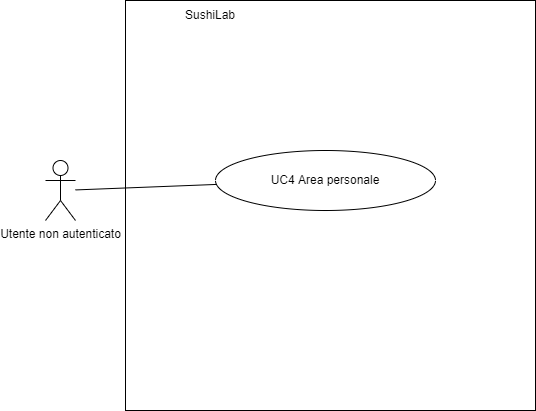
\includegraphics[scale=0.5]{usecase/tesi-uc4.drawio.png}
    \caption{Use Case - UC 4}
\end{figure}
\begin{itemize}
    \item \textbf{Descrizione:} L'utente visualizza la maschera dell'area personale.
    \item \textbf{Attore Primario:}L'utente non autenticato.
    \item \textbf{Precondizione:} L'utente si trova dentro la web-app.
    \item \textbf{Postcondizione:} Viene visualizzata la maschera dell'area personale.
    \item \textbf{Scenario principale:}
    \begin{itemize}
        \item L'utente si trova dentro il sistema;
        \item Viene mostrata la maschera dell'area personale.
    \end{itemize}
\end{itemize}
\textbf{UC4.1 - Registrazione}
\begin{figure}[H]
    \centering
    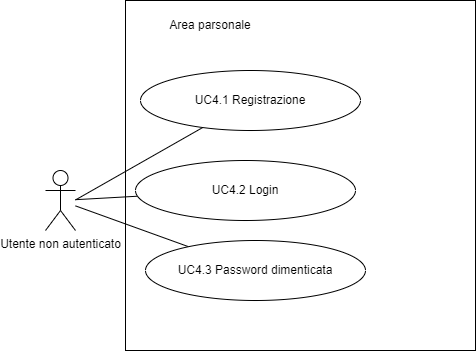
\includegraphics[scale=0.5]{usecase/tesi-uc41.drawio.png}
    \caption{Use Case - UC 4.1, UC 4.2, UC 4.3}
\end{figure}
\begin{itemize}
    \item \textbf{Descrizione:} L'utente viene registrato nella piattaforma.
    \item \textbf{Attore Primario:}L'utente non autenticato.
    \item \textbf{Precondizione:} L'utente si trova dentro la web-app.
    \item \textbf{Postcondizione:} Vengono salvati i dati dell'utente inseriti durante la fase di registrazione nel data-base.
    \item \textbf{Scenario principale:}
    \begin{itemize}
        \item L'utente si trova dentro l'area personale;
        \item L'utente clicca sul bottone registrati;
        \item Viene mostrato il form di registrazione;
        \item L'utente inserisce l'email;
        \item L'utente inserisce la password;
        \item L'utente ripete la password;
        \item L'utente clicca sul bottone registrati;
        \item Viene registrato correttamente l'account.
    \end{itemize}
    % \item \textbf{Estensioni:}
    % \begin{itemize}
    %     \item L'utente inserisce l'email già esistente nel data-base;
    %     \item Non viene registrato l'acocunt.
    % \end{itemize}
\end{itemize}
\textbf{UC4.2 - Login}
\begin{itemize}
    \item \textbf{Descrizione:} L'utente effettua il login nella piattaforma.
    \item \textbf{Attore Primario:} L'utente non autenticato.
    \item \textbf{Precondizione:} L'utente si trova dentro la web-app.
    \item \textbf{Postcondizione:} Viene effettuato il login.
    \item \textbf{Scenario principale:}
    \begin{itemize}
        \item L'utente si trova dentro l'area personale;
        \item L'utente inserisce l'email;
        \item L'utente inserisce la password;
        \item L'utente clicca sul bottone login;
        \item Viene effettuato il login correttamente.
    \end{itemize}
    % \item \textbf{Estensioni:}
    % \begin{itemize}
    %     \item L'utente inserisce l'email non esistente nel data-base o una password errata;
    %     \item Non viene effettuato il login.
    % \end{itemize}
\end{itemize}
\textbf{UC4.3 - Password dimenticata}
\begin{itemize}
    \item \textbf{Descrizione:} L'utente reimposta la password del proprio account.
    \item \textbf{Attore Primario:}L'utente non autenticato.
    \item \textbf{Precondizione:} L'utente si trova dentro la web-app.
    \item \textbf{Postcondizione:} Viene aggiornata la nuova password nel data-base.
    \item \textbf{Scenario principale:}
    \begin{itemize}
        \item L'utente si trova dentro l'area personale;
        \item L'utente clicca sul bottone password dimenticata;
        \item Viene mostrato il form di recupero password;
        \item L'utente inserisce l'email;
        \item L'utente clicca sul bottone ottieni codice;
        \item L'utente arriva nel secondo form tramite il link mandato tramite l'email;
        \item L'utente inserisce la password;
        \item L'utente ripete la password;
        \item L'utente clicca sul bottone cambia password;
        \item Viene cambiata correttamente la password.
    \end{itemize}
    % \item \textbf{Estensioni:}
    % \begin{itemize}
    %     \item L'utente inserisce l'email non esistente nel data-base;
    %     \item Non viene effettuato il cambio password.
    % \end{itemize}
\end{itemize}
% \textbf{UCE1 - Email}
% \begin{itemize}
%     \item \textbf{Descrizione:} L'utente reimposta la password del proprio account.
%     \item \textbf{Attore Primario:}L'utente non autenticato.
%     \item \textbf{Precondizione:} L'utente si trova dentro la web-app.
%     \item \textbf{Postcondizione:} Viene aggiornato la nuova password nel data-base.
%     \item \textbf{Scenario principale:}
%     \begin{itemize}
%         \item L'utente si trova dentro l'area personale;
%         \item L'utente clicca sul bottone password dimenticata;
%         \item Viene mostrato il form di recupero password;
%         \item L'utente inserisce l'email;
%         \item L'utente clicca sul bottone ottieni codice;
%         \item L'utente arriva nel secondo form tramite il link mandato tramite email;
%         \item L'utente inserisce la password;
%         \item L'utente ripete la password;
%         \item L'utente clicca sul bottone cambia password;
%         \item Viene cambiato correttamente la password.
%     \end{itemize}
% \end{itemize}
\textbf{Utente autenticato}\\
\textbf{UC4.4 - Logout}
\begin{figure}[H]
    \centering
    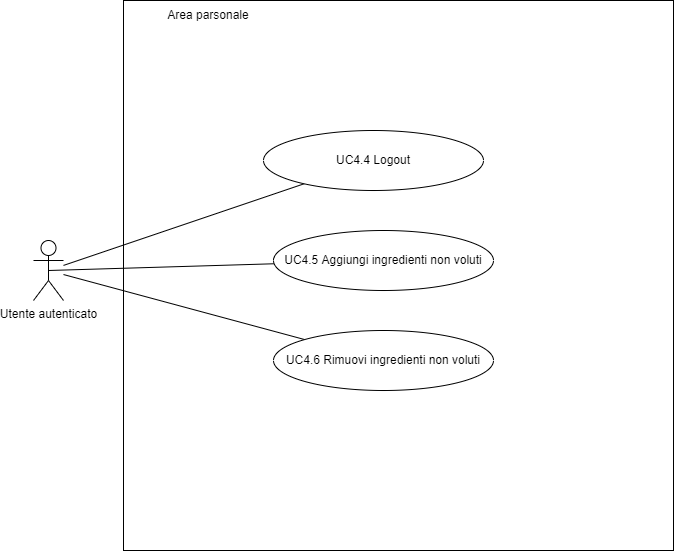
\includegraphics[scale=0.5]{usecase/tesi-uc42.drawio.png}
    \caption{Use Case - UC 4.4, UC4.5, UC4.6}
\end{figure}
\begin{itemize}
    \item \textbf{Descrizione:} L'utente effettua il logout.
    \item \textbf{Attore Primario:}L'utente autenticato.
    \item \textbf{Precondizione:} L'utente si trova dentro la web-app ed ha effettuato il login.
    \item \textbf{Postcondizione:} Viene effettuato il logout.
    \item \textbf{Scenario principale:}
    \begin{itemize}
        \item L'utente si trova dentro l'area personale;
        \item L'utente clicca sul bottone logout;
        \item Viene effettuato il logout dell'utente.
    \end{itemize}
\end{itemize}
\textbf{UC4.5 - Aggiungi ingredienti non voluti}
\begin{itemize}
    \item \textbf{Descrizione:} L'utente inserisce un ingrediente nella blacklist.
    \item \textbf{Attore Primario:}L'utente autenticato.
    \item \textbf{Precondizione:} L'utente si trova dentro la web-app e ha effettuato il login.
    \item \textbf{Postcondizione:} Viene inserito l'ingrediente nella blacklist.
    \item \textbf{Scenario principale:}
    \begin{itemize}
        \item L'utente si trova dentro l'area personale;
        \item L'utente clicca sul bottone blacklist degli ingredienti;
        \item L'utente inserisce il nome dell'ingrediente;
        \item L'utente clicca sul bottone +;
        \item Viene inserito l'ingrediente nella blacklist.
    \end{itemize}
\end{itemize}
\textbf{UC4.6 - Rimuovi ingredienti non voluti}
\begin{itemize}
    \item \textbf{Descrizione:} L'utente rimuove un ingrediente dalla blacklist.
    \item \textbf{Attore Primario:}L'utente autenticato.
    \item \textbf{Precondizione:} L'utente si trova dentro la web-app ed ha effettuato il login.
    \item \textbf{Postcondizione:} Viene rimosso l'ingrediente dalla blacklist.
    \item \textbf{Scenario principale:}
    \begin{itemize}
        \item L'utente si trova dentro l'area personale;
        \item L'utente clicca sul bottone blacklist degli ingredienti;
        \item L'utente clicca sul bottone - di un ingrediente già esistente;
        \item Viene rimosso l'ingrediente dalla blacklist.
    \end{itemize}
\end{itemize}
\textbf{UC1.7 - Aggiungi preferiti}
\begin{figure}[H]
    \centering
    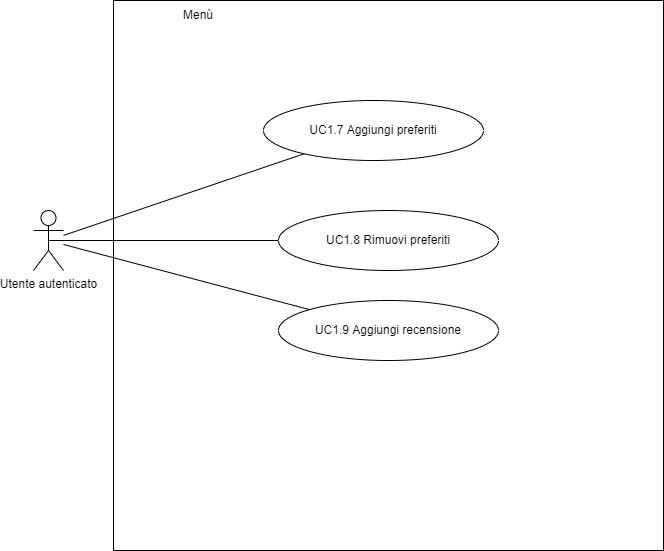
\includegraphics[scale=0.5]{usecase/tesi-uc111.drawio.png}
    \caption{Use Case - UC 1.7, UC1.8, UC1.9}
\end{figure}
\begin{itemize}
    \item \textbf{Descrizione:} L'utente aggiunge un piatto alla lista dei preferiti.
    \item \textbf{Attore Primario:}L'utente autenticato.
    \item \textbf{Precondizione:} L'utente si trova dentro nella sezione menù, lista degli ordini personali o lista degli ordini in arrivo.
    \item \textbf{Postcondizione:} Viene inserito il piatto nei preferiti.
    \item \textbf{Scenario principale:}
    \begin{itemize}
        \item L'utente si trova nella sezione menù, lista degli ordini personali o lista degli ordini in arrivo;
        \item L'utente clicca sul bottone "cuore grigio";
        \item Viene inserito il piatto nella lista dei preferiti.
    \end{itemize}
\end{itemize}
\textbf{UC1.8 - Rimuovi preferiti}
\begin{itemize}
    \item \textbf{Descrizione:} L'utente rimuove un piatto dalla lista dei preferiti.
    \item \textbf{Attore Primario:}L'utente autenticato.
    \item \textbf{Precondizione:} L'utente si trova dentro nella sezione menù, lista degli ordini personali, lista degli ordini in arrivo o lista preferiti.
    \item \textbf{Postcondizione:} Viene rimosso il piatto dalla lista dei preferiti.
    \item \textbf{Scenario principale:}
    \begin{itemize}
        \item L'utente si trova nella sezione menù;
        \item L'utente clicca sul bottone "cuore rosa";
        \item Viene rimosso il piatto dalla lista dei preferiti.
    \end{itemize}
\end{itemize}
\textbf{UC1.9 - Aggiungi recensione}
\begin{itemize}
    \item \textbf{Descrizione:} L'utente aggiunge una recensione per un piatto.
    \item \textbf{Attore Primario:}L'utente autenticato.
    \item \textbf{Precondizione:} L'utente ha selezionato un piatto in modalità dettaglio.
    \item \textbf{Postcondizione:} Viene aggiornata la recensione del piatto.
    \item \textbf{Scenario principale:}
    \begin{itemize}
        \item L'utente ha selezionato un piatto in modalità dettaglio;
        \item L'utente clicca su una delle 5 stelle;
        \item Viene inserita la recensione del piatto.
    \end{itemize}
\end{itemize}
\textbf{UC5 - Visualizza lista preferiti}
\begin{figure}[H]
    \centering
    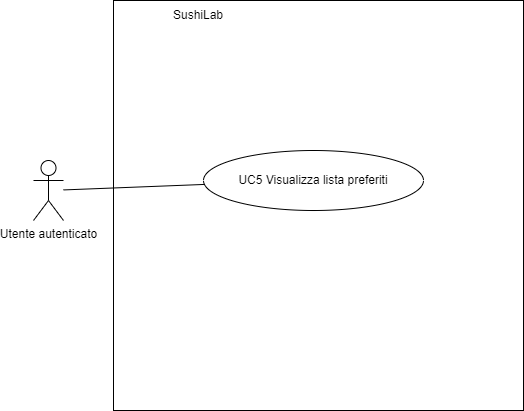
\includegraphics[scale=0.5]{usecase/tesi-uc5.drawio.png}
    \caption{Use Case - UC 5}
\end{figure}
\begin{itemize}
    \item \textbf{Descrizione:} L'utente visualizza la lista dei preferiti.
    \item \textbf{Attore Primario:}L'utente autenticato.
    \item \textbf{Precondizione:} L'utente si trova dentro la web-app ed ha effettuato il login.
    \item \textbf{Postcondizione:} Viene mostrata la lista dei preferiti.
    \item \textbf{Scenario principale:}
    \begin{itemize}
        \item L'utente si trova dentro la web-app;
        \item L'utente entra nalla sezione lista preferiti;
        \item Viene mostrata la lista dei preferiti.
    \end{itemize}
\end{itemize}
             % Appendice A

%**************************************************************
% Materiale finale
%**************************************************************
\backmatter
\printglossaries
\input{inizio-fine/bibliografia}
\end{document}
